% !TeX program = xelatex
\documentclass[a4paper,12pt]{article}

% ============================================================================
% មគ្គុទ្ទេសក៍គរុកោសល្យគ្រូ និងរបាយការណ៍ស្រាវជ្រាវសង្ខេប (Teaching Guideline & Mini-Research Report)
% មេរៀនទី១២៖ ១.២.២ មុំមួយប៉ុនគ្នាអមដោយជ្រុងពីរប៉ុនរៀងគ្នា — ករណី ជ.ម.ជ (SAS)
% ត្រូវគ្នា ១០០% នឹង LS_Plan_SAS.tex, Teaching_Scenario_SAS.tex, Printable_Materials_SAS.tex
% និងអត្ថបទស្រាវជ្រាវ Open-Access ទាំង ១៤ ក្នុង ឯកសារស្រាវជ្រាវយោង_PDF\
% ============================================================================
\usepackage[a4paper, left=1.45cm, right=1.45cm, top=2.30cm, bottom=2.30cm, headheight=18pt, headsep=0.68cm, footskip=0.88cm]{geometry}
\usepackage{amsmath, amssymb}
\usepackage{unicode-math}
\usepackage{fontspec}
\usepackage{array, longtable, multirow, colortbl, booktabs}
\usepackage[table]{xcolor}
\usepackage{enumitem}
\usepackage{pifont}
\usepackage{fancyhdr}
\usepackage{lastpage}
\usepackage{needspace}
\usepackage[hyphens]{url}
\usepackage{tikz}
\usepackage[most]{tcolorbox}
\usetikzlibrary{calc, arrows.meta, angles, quotes, decorations.markings, positioning, babel}
\urlstyle{same}

% LaTeX 2025 + longtable compatibility guard
\makeatletter
\let\@expl@@@mark@update@singlecol@structures@@\relax
\makeatother

% ============================================================================
% ការកំណត់ពុម្ពអក្សរ (Word-Styled Khmer + Times New Roman APA + Cambria Math)
% ============================================================================
% Cross-platform font path resolver (Windows local + Linux/Cloud repo fonts/)
\providecommand{\NGSFindFonts}{%
  \IfFileExists{C:/Windows/Fonts/cambria.ttc}{%
    \def\NGSSysPath{C:/Windows/Fonts/}%
    \def\NGSUserPath{C:/Users/KIT/AppData/Local/Microsoft/Windows/Fonts/}%
  }{%
    \IfFileExists{./fonts/KhmerOSsiemreap.ttf}{\def\NGSSysPath{./fonts/}\def\NGSUserPath{./fonts/}}{%
    \IfFileExists{../fonts/KhmerOSsiemreap.ttf}{\def\NGSSysPath{../fonts/}\def\NGSUserPath{../fonts/}}{%
    \IfFileExists{../../fonts/KhmerOSsiemreap.ttf}{\def\NGSSysPath{../../fonts/}\def\NGSUserPath{../../fonts/}}{%
    \IfFileExists{../../../fonts/KhmerOSsiemreap.ttf}{\def\NGSSysPath{../../../fonts/}\def\NGSUserPath{../../../fonts/}}{%
    \IfFileExists{../../../../fonts/KhmerOSsiemreap.ttf}{\def\NGSSysPath{../../../../fonts/}\def\NGSUserPath{../../../../fonts/}}{%
    \IfFileExists{../../../../../fonts/KhmerOSsiemreap.ttf}{\def\NGSSysPath{../../../../../fonts/}\def\NGSUserPath{../../../../../fonts/}}{%
    \IfFileExists{../../../../../../fonts/KhmerOSsiemreap.ttf}{\def\NGSSysPath{../../../../../../fonts/}\def\NGSUserPath{../../../../../../fonts/}}{%
      \def\NGSSysPath{../../../../../../../fonts/}\def\NGSUserPath{../../../../../../../fonts/}%
    }}}}}}}%
  }%
}
\NGSFindFonts

\setmathfont[
  Path={\NGSSysPath},
  FontIndex=1,
  Scale=1.06
]{cambria.ttc}

\defaultfontfeatures{Ligatures=TeX}

\setmainfont[
  Path={\NGSUserPath},
  Extension=.ttf,
  Script=Khmer,
  BoldFont={KhmerOSsiemreap},
  BoldFeatures={FakeBold=1.8},
  ItalicFont={KhmerOSsiemreap},
  ItalicFeatures={FakeSlant=0.25},
  BoldItalicFont={KhmerOSsiemreap},
  BoldItalicFeatures={FakeBold=1.8, FakeSlant=0.25}
]{KhmerOSsiemreap}

\newfontfamily\muol[
  Path={\NGSUserPath},
  Extension=.ttf,
  Script=Khmer
]{KhmerOSmuollight}

\newfontfamily\TimesEn[
  Path={\NGSSysPath},
  Extension=.ttf,
  Scale=1.02,
  BoldFont={timesbd},
  ItalicFont={timesi},
  BoldItalicFont={timesbi}
]{times}

\newfontfamily\CalibriFont[
  Path={\NGSSysPath},
  Extension=.ttf
]{calibri}

\newfontfamily\Tacteing[
  Path={\NGSUserPath}
]{TACTENG.TTF}

\newfontfamily\CourierBullet[
  Path={\NGSSysPath},
  Extension=.ttf
]{cour}

% ក្បួនកាត់ពាក្យខ្មែរ (Khmer word wrapping)
\XeTeXlinebreaklocale "km"
\XeTeXlinebreakskip = 0pt plus 1pt minus 0.1pt

% ============================================================================
% ពណ៌បោះពុម្ព ស-ខ្មៅ / ប្រផេះ (Strict Print-Safe Monochrome & Grayscale)
% ============================================================================
\definecolor{headgray}{HTML}{F2F2F2}
\definecolor{panelgray}{gray}{0.94}
\definecolor{stepgray}{HTML}{D9D9D9}
\definecolor{midgray}{gray}{0.82}
\definecolor{bordergray}{gray}{0.45}

\pagestyle{fancy}
\fancyhf{}
\renewcommand{\headrulewidth}{0.4pt}
\renewcommand{\footrulewidth}{0.4pt}
\fancyhead[L]{\rule[-3pt]{0pt}{14pt}\fontsize{9.5pt}{14pt}\selectfont អនុវិទ្យាល័យព្រះក្រសាំង — មគ្គុទ្ទេសក៍គរុកោសល្យគ្រូ \en{(Grade 8 SAS)}}
\fancyhead[R]{\rule[-3pt]{0pt}{14pt}\fontsize{9.5pt}{14pt}\selectfont មេរៀនទី១២ (១.២.២) ករណី ជ.ម.ជ \en{(SAS)}}
\fancyfoot[L]{\rule{0pt}{13pt}\fontsize{9.5pt}{14pt}\selectfont កញ្ចប់ឯកសារ \en{NGS 5Es} (៥០ នាទី) | ហុក ប៊ុនថែន}
\fancyfoot[R]{\rule{0pt}{13pt}\fontsize{9.5pt}{14pt}\selectfont ទំព័រ \en{\thepage\ / \pageref{LastPage}}}

\fancypagestyle{firstpage}{%
  \fancyhf{}%
  \renewcommand{\headrulewidth}{0pt}%
  \renewcommand{\footrulewidth}{0.4pt}%
  \fancyfoot[L]{\rule{0pt}{13pt}\fontsize{9.5pt}{14pt}\selectfont កញ្ចប់ឯកសារ \en{NGS 5Es} (៥០ នាទី) | អនុវិទ្យាល័យព្រះក្រសាំង}%
  \fancyfoot[R]{\rule{0pt}{13pt}\fontsize{9.5pt}{14pt}\selectfont ទំព័រ \en{\thepage\ / \pageref{LastPage}}}%
}

\setlength{\parindent}{0pt}
\setlength{\parskip}{4.5pt}
\setlength{\tabcolsep}{4pt}
\setlength{\emergencystretch}{2em}
\setlist{itemsep=4pt, parsep=0pt}

% ============================================================================
% ម៉ាក្រូជំនួយ (Helper Macros)
% ============================================================================
\newcommand{\en}[1]{{\TimesEn #1}}
\newcommand{\enbf}[1]{{\TimesEn\textbf{#1}}}
\newcommand{\enit}[1]{{\TimesEn\textit{#1}}}
\newcommand{\unit}[1]{\,\text{\en{#1}}}
\newcommand{\cnum}[1]{{\fontsize{10.5pt}{12pt}\selectfont\ding{\numexpr181+#1\relax}}}
\newcommand{\ditem}{\tikz[baseline=-0.5ex]\fill (0,0.40ex) -- (0.40ex,0) -- (0,-0.40ex) -- (-0.40ex,0) -- cycle;\hspace{0.25em}}
\newcommand{\wcirc}{{\CourierBullet\fontsize{9.5pt}{11pt}\selectfont o}}
\newcommand{\tri}[1]{\ensuremath{\triangle #1}}
\newcommand{\ang}[1]{\ensuremath{\angle #1}}
\newcommand{\cg}{\ensuremath{\cong}}
\newcommand{\ncg}{\ensuremath{\not\cong}}
\newcommand{\khmflourish}{{\Tacteing\fontsize{38pt}{15pt}\selectfont\raisebox{-5pt}{3}}}
\newcommand{\tickone}{\tikz[baseline=-0.2ex]\draw[black, line width=1.1pt] (0,0) -- (0,0.24cm);}
\newcommand{\ticktwo}{\tikz[baseline=-0.2ex]{\draw[black, line width=1.1pt] (0,0) -- (0,0.24cm);\draw[black, line width=1.1pt] (0.08cm,0) -- (0.08cm,0.24cm);}}

\newcolumntype{L}[1]{>{\raggedright\arraybackslash}p{#1}}
\newcolumntype{C}[1]{>{\centering\arraybackslash}p{#1}}

% ក្បាលផ្នែកសំខាន់ៗ (Tier 2 — Two-Line Stacked Unwrapped \muol Banner)
\newcommand{\secbanner}[2]{%
  \needspace{2.2cm}%
  \vspace{4pt}%
  \begin{tcolorbox}[
    enhanced, sharp corners, colback=stepgray, colframe=black,
    boxrule=1.1pt, borderline south={0.6pt}{1.8pt}{black},
    top=6pt, bottom=6pt, left=9pt, right=9pt,
    before skip=10pt, after skip=8pt
  ]
    {\muol\fontsize{12pt}{19pt}\selectfont #1}\\[2pt]
    {\fontsize{10pt}{14.5pt}\selectfont\enit{#2}}%
  \end{tcolorbox}%
}

% ក្បាលឯកសារយោងសង្ខេប
\newcommand{\refbanner}[1]{%
  \needspace{2.2cm}%
  \vspace{4pt}%
  \begin{tcolorbox}[
    enhanced, sharp corners, colback=stepgray, colframe=black,
    boxrule=1.1pt, borderline south={0.6pt}{1.8pt}{black},
    top=6pt, bottom=6pt, left=9pt, right=9pt,
    before skip=10pt, after skip=8pt
  ]
    {\muol\fontsize{12pt}{19pt}\selectfont #1}%
  \end{tcolorbox}%
}

% ចំណងជើងផ្នែករង (Tier 3 — Unwrapped \muol + Subtle Bottom Rule)
\newcommand{\subsec}[1]{%
  \Needspace{1.3cm}%
  \vspace{0pt}%
  {\muol\fontsize{11.5pt}{18.5pt}\selectfont #1}\par
  \vspace{1pt}\hrule height 0.5pt\vspace{2pt}%
}

% ប្រអប់ដំណាក់កាល ៥ នាទី-ទល់-នាទី (Top Header Bar + Breakable Body for Inner scriptbox)
\newenvironment{phasebox}[3]{%
  \needspace{2.2cm}%
  \begin{tcolorbox}[
    enhanced, sharp corners, colback=headgray, colframe=black,
    boxrule=1.0pt, top=4pt, bottom=4pt, left=9pt, right=9pt,
    before skip=7pt, after skip=3pt
  ]%
    \renewcommand{\arraystretch}{1.0}%
    \begin{tabular*}{\linewidth}{@{}>{\raggedright\arraybackslash}p{13.60cm}@{\extracolsep{\fill}}r@{}}
      {\muol\fontsize{11pt}{17.5pt}\selectfont #1} & {\fontsize{10.5pt}{15pt}\selectfont\en{#2 |} #3}%
    \end{tabular*}%
  \end{tcolorbox}%
  \begingroup\fontsize{11.5pt}{18.2pt}\selectfont
}{%
  \par\endgroup\vspace{3pt}\hrule height 0.5pt\vspace{5pt}%
}

% ប្រអប់ពាក្យសម្ដីគ្រូនិយាយផ្ទាល់ (Tier 4 Body 11.5pt/18.2pt)
\newtcolorbox{scriptbox}{%
  enhanced, breakable, sharp corners, colback=panelgray, colframe=black,
  boxrule=0.6pt, borderline west={2.4pt}{0pt}{black},
  top=5pt, bottom=5pt, left=9pt, right=8pt,
  before skip=4pt, after skip=4pt,
  fontupper=\fontsize{11.5pt}{18.2pt}\selectfont
}

% រចនាប័ទ្មគូសសម្គាល់ជ្រុងស្មើគ្នា (B&W Print-Safe TikZ Tick Marks >=1.0pt)
\tikzset{
  tk1/.style={postaction={decorate},decoration={markings,
    mark=at position 0.50 with {\draw[black, line width=1.05pt](0,-0.10)--(0,0.10);}}},
  tk2/.style={postaction={decorate},decoration={markings,
    mark=at position 0.44 with {\draw[black, line width=1.05pt](0,-0.10)--(0,0.10);},
    mark=at position 0.56 with {\draw[black, line width=1.05pt](0,-0.10)--(0,0.10);}}}
}

% ============================================================================
% រូបភាពធរណីមាត្រ TikZ ស-ខ្មៅ គុណភាពខ្ពស់ (4 Crisp B&W Pedagogical Diagrams)
% ============================================================================

% រូបទី ១៖ គំរូវាស់ទទឹងស្រះទឹកប្រយោលនៅអនុវិទ្យាល័យព្រះក្រសាំង (E1 Engage -> E5 Closure)
\newcommand{\figGuidelinePond}{%
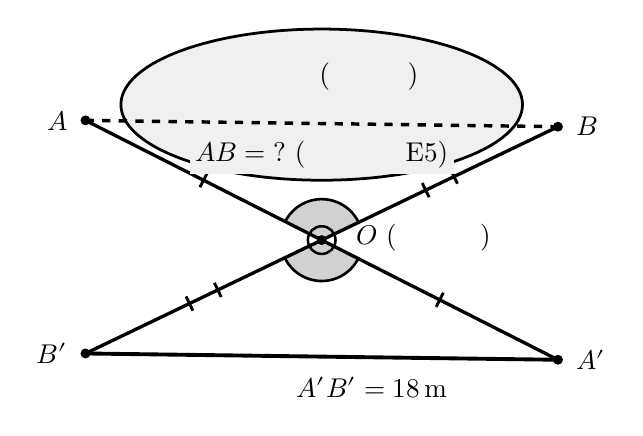
\begin{tikzpicture}[x=1cm, y=1cm, every node/.style={font=\fontsize{9.8pt}{14pt}\selectfont, text=black}]
  \coordinate (O) at (0,0);
  \coordinate (A) at (-3.0, 1.52);
  \coordinate (B) at (3.0, 1.44);
  \coordinate (Ap) at (3.0, -1.52);
  \coordinate (Bp) at (-3.0, -1.44);

  % ស្រះទឹកប្រផេះស្រាល (ស-ខ្មៅ)
  \fill[panelgray, draw=black, line width=1.0pt] (0, 1.72) ellipse (2.55 and 0.96);
  \node[font=\fontsize{10pt}{14.5pt}\selectfont] at (0, 2.08) {\textbf{ស្រះទឹកសាលា} (ឆ្លងមិនរួច)};

  % ធ្នូមុំទល់កំពូលត្រង់ O
  \fill[midgray] (O) -- ($(O)+(153:0.52)$) arc (153:25.6:0.52) -- cycle;
  \fill[midgray] (O) -- ($(O)+(-27:0.52)$) arc (-27:-154.4:0.52) -- cycle;
  \draw[black, line width=0.95pt] ($(O)+(153:0.52)$) arc (153:25.6:0.52);
  \draw[black, line width=0.95pt] ($(O)+(-27:0.52)$) arc (-27:-154.4:0.52);
  \draw[black, line width=0.9pt] (O) circle (5pt);

  % ខ្សែតម្រង់កាត់គ្នា និងជ្រុងស្មើគ្នា
  \draw[black, line width=1.2pt, tk1] (A) -- (O);
  \draw[black, line width=1.2pt, tk1] (O) -- (Ap);
  \draw[black, line width=1.2pt, tk2] (B) -- (O);
  \draw[black, line width=1.2pt, tk2] (O) -- (Bp);

  % ចម្ងាយមិនស្គាល់ AB និងចម្ងាយវាស់លើគោក A'B'
  \draw[black, line width=1.25pt, dashed] (A) -- (B);
  \draw[black, line width=1.4pt] (Bp) -- (Ap);

  \fill[black] (O) circle (1.8pt) (A) circle (1.8pt) (B) circle (1.8pt) (Ap) circle (1.8pt) (Bp) circle (1.8pt);
  \node[right=9pt, yshift=1pt] at (O) {$O$ (បង្គោលផ្ចិត)};
  \node[left=3pt] at (A) {$A$};
  \node[right=3pt] at (B) {$B$};
  \node[right=3pt] at (Ap) {$A'$};
  \node[left=3pt] at (Bp) {$B'$};
  \node[fill=panelgray, inner sep=2pt] at (0, 1.08) {$AB = \text{?}$ (សន្និដ្ឋាននៅ \en{E5})};
  \node[below=4pt] at ($(Bp)!0.5!(Ap)$) {\textbf{វាស់លើដីគោក៖} $A'B' = 18\unit{m}$};
\end{tikzpicture}}

% រូបទី ២៖ ការប្រៀបធៀប SAS 60° (រាងតែមួយគត់) ទល់នឹង អន្ទាក់ SSA 32° (កើតជា C1, C2)
\newcommand{\figGuidelineHingeVsSSA}{%
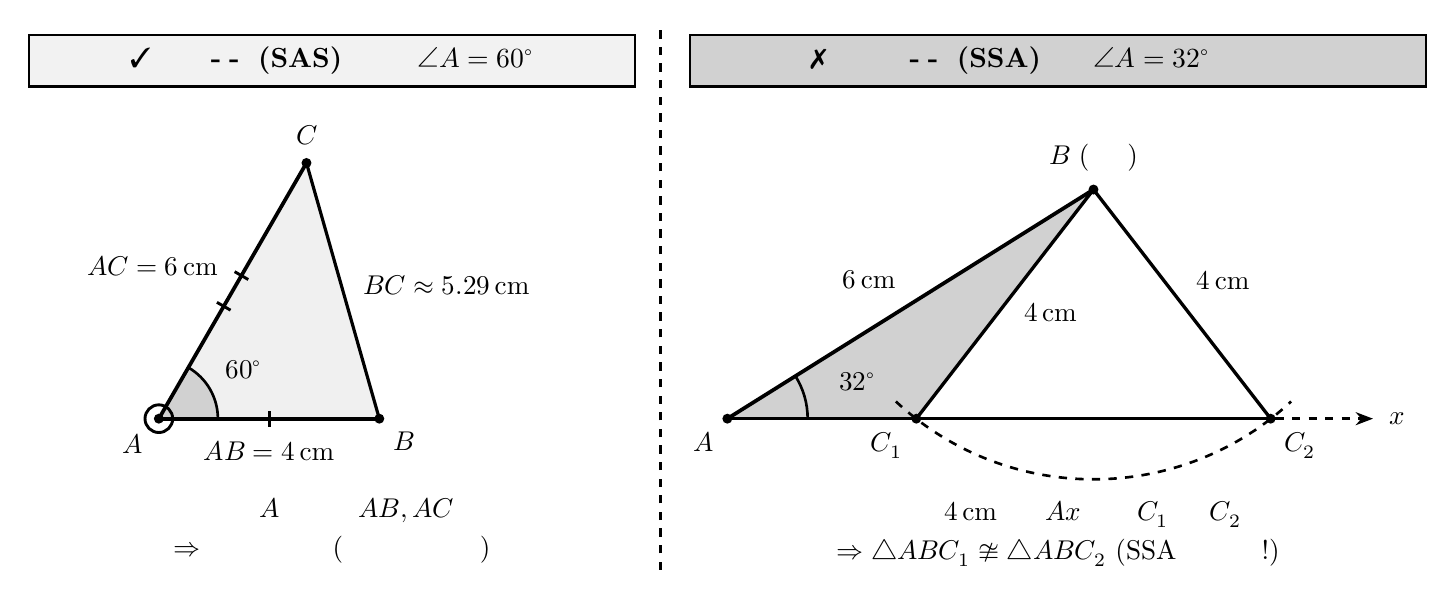
\begin{tikzpicture}[x=1cm, y=1cm, every node/.style={font=\fontsize{9.8pt}{14pt}\selectfont, text=black}]
  % ផ្នែកឆ្វេង៖ SAS 60 deg (Unique) — x: 0.05..7.85 cm
  \begin{scope}[shift={(0.05, 0)}]
    \node[draw=black, fill=headgray, line width=0.9pt, minimum width=7.70cm, minimum height=0.66cm, anchor=south, font=\fontsize{10pt}{14.5pt}\selectfont] at (3.90, 4.50) {\textbf{\ding{51}\ ករណី ជ-ម-ជ (\en{SAS})៖ ចាក់សោ $\ang{A}=60^\circ$}};
    \coordinate (A) at (1.70, 0.30);
    \coordinate (B) at (4.50, 0.30);
    \coordinate (C) at ($(A)+(60:3.75)$);
    \fill[panelgray] (A) -- (B) -- (C) -- cycle;
    \fill[midgray] (A) -- ($(A)+(0.75,0)$) arc (0:60:0.75) -- cycle;
    \draw[black, line width=0.95pt] ($(A)+(0.75,0)$) arc (0:60:0.75);
    \draw[black, line width=1.05pt] (A) circle (5pt);
    \draw[black, line width=1.35pt, tk1] (A) -- (B) node[midway, below=4pt] {$AB = 4\unit{cm}$};
    \draw[black, line width=1.35pt, tk2] (A) -- (C) node[midway, above left=2pt] {$AC = 6\unit{cm}$};
    \draw[black, line width=1.15pt] (B) -- (C) node[pos=0.52, right=4pt] {$BC \approx 5.29\unit{cm}$};
    \node at ($(A)+(30:1.25)$) {$60^\circ$};
    \fill[black] (A) circle (1.8pt) (B) circle (1.8pt) (C) circle (1.8pt);
    \node[below left=3pt] at (A) {$A$};
    \node[below right=2pt] at (B) {$B$};
    \node[above=3pt] at (C) {$C$};
    \node[align=center] at (3.90, -1.12) {កំពូល $A$ នៅចន្លោះ $AB, AC$\\$\Rightarrow$ ត្រីកោណ\textbf{តែមួយគត់} (ត្រួតស៊ីគ្នាបេះបិទ)};
  \end{scope}

  % បន្ទាត់បំបែកកណ្ដាល
  \draw[black, dashed, line width=0.9pt] (8.12, -1.62) -- (8.12, 5.25);

  % ផ្នែកស្ដាំ៖ SSA 32 deg (Ambiguous C1, C2) — x: 8.40..17.95 cm
  \begin{scope}[shift={(8.42, 0)}]
    \node[draw=black, fill=midgray, line width=0.9pt, minimum width=9.35cm, minimum height=0.66cm, anchor=south, font=\fontsize{10pt}{14.5pt}\selectfont] at (4.75, 4.50) {\textbf{\ding{55}\ អន្ទាក់ ជ-ជ-ម (\en{SSA})៖ មុំ $\ang{A}=32^\circ$ មិននៅចន្លោះ}};
    \coordinate (A) at (0.55, 0.30);
    \coordinate (B) at (5.20, 3.21);
    \coordinate (C1) at (2.95, 0.30);
    \coordinate (C2) at (7.45, 0.30);
    \coordinate (Xend) at (8.75, 0.30);
    \fill[midgray] (A) -- (B) -- (C1) -- cycle;
    \fill[white] (B) -- (C1) -- (C2) -- cycle;
    \draw[black, line width=1.0pt, dashed, -{Stealth[length=2.2mm]}] (A) -- (Xend) node[right=2pt] {$x$};
    \draw[black, line width=1.35pt] (A) -- (B) node[midway, above left=2pt] {$6\unit{cm}$};
    \draw[black, line width=1.2pt] (B) -- (C1) node[midway, right=3pt, yshift=-3pt] {$4\unit{cm}$};
    \draw[black, line width=1.2pt] (B) -- (C2) node[midway, above right=2pt] {$4\unit{cm}$};
    \draw[black, line width=1.1pt] (A) -- (C2);
    \draw[black, line width=0.95pt, dashed] ($(B)+(-133:3.68)$) arc (-133:-47:3.68);
    \draw[black, line width=0.95pt] ($(A)+(1.02, 0)$) arc (0:32:1.02);
    \node at ($(A)+(16:1.72)$) {$32^\circ$};
    \fill[black] (A) circle (1.8pt) node[below left=2pt] {$A$};
    \fill[black] (B) circle (1.8pt) node[above=3pt] {$B$ (ម្ជុល)};
    \fill[black] (C1) circle (1.8pt) node[below left=2pt] {$C_1$};
    \fill[black] (C2) circle (1.8pt) node[below right=2pt] {$C_2$};
    \node[align=center] at (4.75, -1.16) {យោលបន្ទះ $4\unit{cm}$ កាត់ $Ax$ ត្រង់ $C_1$ និង $C_2$\\$\Rightarrow \tri{ABC_1} \ncg \tri{ABC_2}$ (\en{SSA} ប្រើមិនបាន!)};
  \end{scope}
\end{tikzpicture}}

% រូបទី ៣៖ វិធីគូសសញ្ញា ស-ខ្មៅ & ចង្អុលម្រាមដៃ ៣ ជំហាន (E4 កាតទី ១)
\newcommand{\figGuidelineThreeStep}{%
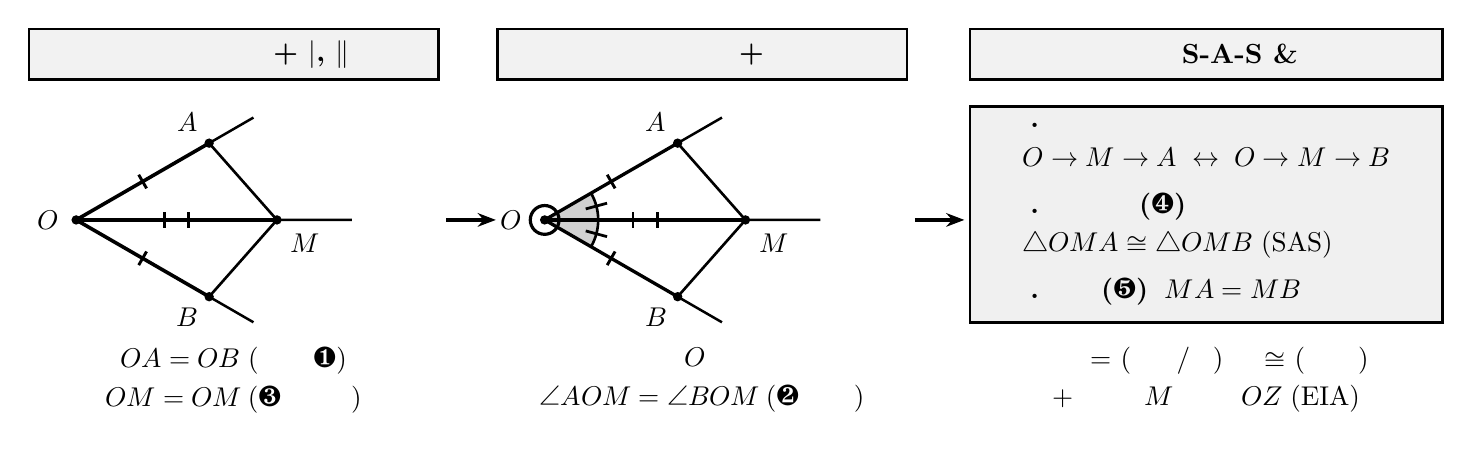
\begin{tikzpicture}[x=1cm, y=1cm, every node/.style={font=\fontsize{9.8pt}{14pt}\selectfont, text=black}]
  % ជំហានទី ១ (x: 0.0..5.25)
  \begin{scope}[shift={(0.0, 0)}]
    \node[draw=black, fill=headgray, line width=0.9pt, minimum width=5.20cm, minimum height=0.64cm, anchor=south, font=\fontsize{10pt}{14.5pt}\selectfont] at (2.55, 2.85) {\textbf{ជំហាន ១៖ ចង្អុលអូស + $|$, $\parallel$}};
    \coordinate (O) at (0.55, 1.08);
    \coordinate (X) at (30:2.60);
    \coordinate (Y) at (-30:2.60);
    \coordinate (Z) at (4.05, 1.08);
    \coordinate (A) at ($(O)+(30:1.95)$);
    \coordinate (B) at ($(O)+(-30:1.95)$);
    \coordinate (M) at (3.10, 1.08);
    \draw[black, line width=0.9pt] (A) -- ($(O)+(X)$) (B) -- ($(O)+(Y)$) (M) -- (Z);
    \draw[black, line width=1.3pt, tk1] (O) -- (A);
    \draw[black, line width=1.3pt, tk1] (O) -- (B);
    \draw[black, line width=1.4pt, tk2] (O) -- (M);
    \draw[black, line width=0.95pt] (A) -- (M) -- (B);
    \fill[black] (O) circle (1.7pt) (A) circle (1.7pt) (B) circle (1.7pt) (M) circle (1.7pt);
    \node[left=3pt] at (O) {$O$};
    \node[above left=1pt] at (A) {$A$};
    \node[below left=1pt] at (B) {$B$};
    \node[below right=2pt] at (M) {$M$};
    \node[align=center] at (2.55, -0.95) {$OA=OB$ (ហេតុផល \cnum{1})\\$OM=OM$ (\cnum{3} ជ្រុងរួម)};
  \end{scope}

  \draw[black, line width=1.2pt, -{Stealth[length=2.3mm]}] (5.25, 1.08) -- (5.88, 1.08);

  % ជំហានទី ២ (x: 5.95..11.20)
  \begin{scope}[shift={(5.95, 0)}]
    \node[draw=black, fill=headgray, line width=0.9pt, minimum width=5.20cm, minimum height=0.64cm, anchor=south, font=\fontsize{10pt}{14.5pt}\selectfont] at (2.55, 2.85) {\textbf{ជំហាន ២៖ ព័ទ្ធកំពូល + ធ្នូមុំ}};
    \coordinate (O) at (0.55, 1.08);
    \coordinate (X) at (30:2.60);
    \coordinate (Y) at (-30:2.60);
    \coordinate (Z) at (4.05, 1.08);
    \coordinate (A) at ($(O)+(30:1.95)$);
    \coordinate (B) at ($(O)+(-30:1.95)$);
    \coordinate (M) at (3.10, 1.08);
    \fill[midgray] (O) -- ($(O)+(30:0.68)$) arc (30:-30:0.68) -- cycle;
    \draw[black, line width=0.95pt] ($(O)+(30:0.68)$) arc (30:-30:0.68);
    \draw[black, line width=1.0pt] ($(O)+(15:0.54)$) -- ($(O)+(15:0.82)$);
    \draw[black, line width=1.0pt] ($(O)+(-15:0.54)$) -- ($(O)+(-15:0.82)$);
    \draw[black, line width=1.15pt] (O) circle (5.2pt);
    \draw[black, line width=0.9pt] (A) -- ($(O)+(X)$) (B) -- ($(O)+(Y)$) (M) -- (Z);
    \draw[black, line width=1.2pt, tk1] (O) -- (A);
    \draw[black, line width=1.2pt, tk1] (O) -- (B);
    \draw[black, line width=1.3pt, tk2] (O) -- (M);
    \draw[black, line width=0.95pt] (A) -- (M) -- (B);
    \fill[black] (O) circle (1.7pt) (A) circle (1.7pt) (B) circle (1.7pt) (M) circle (1.7pt);
    \node[left=5pt] at (O) {$O$};
    \node[above left=1pt] at (A) {$A$};
    \node[below left=1pt] at (B) {$B$};
    \node[below right=2pt] at (M) {$M$};
    \node[align=center] at (2.55, -0.95) {កំពូលរួម $O$ ជាប់ចន្លោះ\\$\ang{AOM}=\ang{BOM}$ (\cnum{2} ពុះមុំ)};
  \end{scope}

  \draw[black, line width=1.2pt, -{Stealth[length=2.3mm]}] (11.20, 1.08) -- (11.83, 1.08);

  % ជំហានទី ៣ (x: 11.90..17.95)
  \begin{scope}[shift={(11.90, 0)}]
    \node[draw=black, fill=headgray, line width=0.9pt, minimum width=6.00cm, minimum height=0.64cm, anchor=south, font=\fontsize{10pt}{14.5pt}\selectfont] at (3.00, 2.85) {\textbf{ជំហាន ៣៖ ផ្ទៀង \en{S-A-S} \& លំដាប់}};
    \draw[black, fill=panelgray, line width=0.95pt] (0.00, -0.22) rectangle (6.00, 2.52);
    \node[align=left] at (3.00, 1.15) {%
      \textbf{១. លំដាប់ឆ្លងត្រីកោណ៖}\\
      $O \to M \to A \;\leftrightarrow\; O \to M \to B$\\[3pt]
      \textbf{២. សន្និដ្ឋាន (\cnum{4})៖}\\
      $\tri{OMA} \cg \tri{OMB}$ (\en{SAS})\\[3pt]
      \textbf{៣. វិបាក (\cnum{5})៖} $MA = MB$%
    };
    \node[align=center] at (3.00, -0.95) {រក្សា $=$ (ប្រវែង/មុំ) ទល់ $\cg$ (ត្រីកោណ)\\+ ពិនិត្យ $M$ រំកិលលើ $OZ$ (\en{EIA})};
  \end{scope}
\end{tikzpicture}}

% រូបទី ៤៖ លំហូរការងារប្រលង Relay ៣ តួនាទី និងចំណុចផ្អាក Pause-Ask / Pause-Review (E5)
\newcommand{\figGuidelineRelay}{%
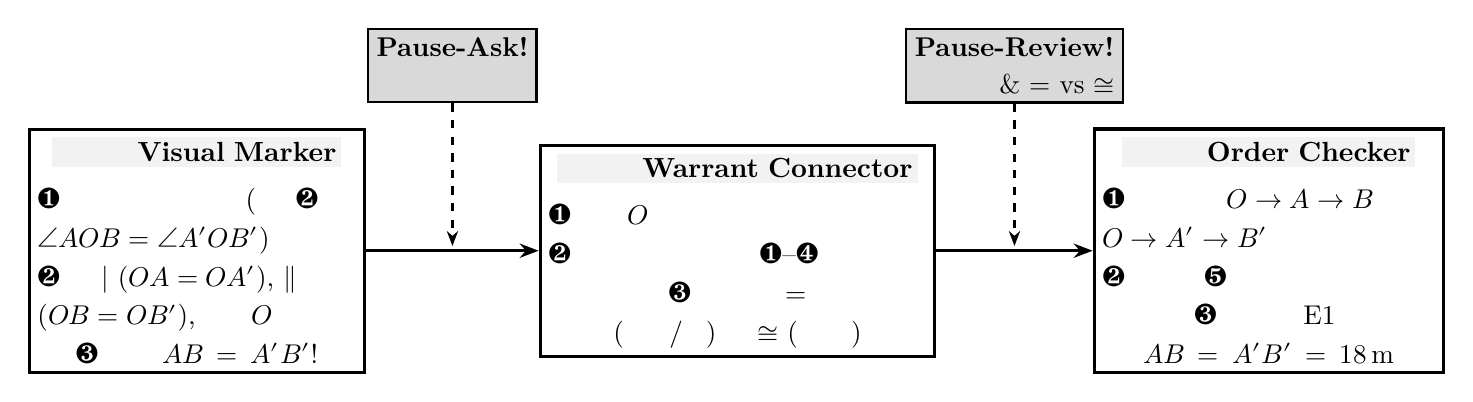
\begin{tikzpicture}[x=0.992cm, y=1cm, every node/.style={font=\fontsize{9.8pt}{14pt}\selectfont, text=black}]
  % តួនាទី ១ (x: 0.00..4.26)
  \node[draw=black, fill=white, line width=1.1pt, text width=4.05cm, align=center, inner sep=3pt] (r1) at (2.13, 0) {%
    {\setlength{\fboxsep}{1.8pt}\colorbox{headgray}{\fontsize{10pt}{14.5pt}\selectfont\textbf{តួនាទី ១៖ \en{Visual Marker}}}}\\[3pt]
    \raggedright\fontsize{9.8pt}{14pt}\selectfont
    \cnum{1} ពន្យល់មាត់ផ្ទាល់មុនគូស (ចាប់ \cnum{2} $\ang{AOB}=\ang{A'OB'}$)\\
    \cnum{2} គូស $|$ ($OA=OA'$), $\parallel$ ($OB=OB'$), ព័ទ្ធ $O$\\
    \cnum{3} \textbf{ហាមគូស} $AB=A'B'$!%
  };

  % តួនាទី ២ (x: 6.55..11.55)
  \node[draw=black, fill=white, line width=1.1pt, text width=4.80cm, align=center, inner sep=3pt] (r2) at (9.05, 0) {%
    {\setlength{\fboxsep}{1.8pt}\colorbox{headgray}{\fontsize{10pt}{14.5pt}\selectfont\textbf{តួនាទី ២៖ \en{Warrant Connector}}}}\\[3pt]
    \raggedright\fontsize{9.8pt}{14pt}\selectfont
    \cnum{1} ផ្ទៀង $O$ នៅចន្លោះជ្រុងទាំងពីរ\\
    \cnum{2} សរសេរ ៣ បន្ទាត់ដាក់លេខ \cnum{1}--\cnum{4}\\
    \cnum{3} រក្សាសញ្ញា $=$ (ប្រវែង/មុំ) និង $\cg$ (ត្រីកោណ)%
  };

  % តួនាទី ៣ (x: 13.63..18.06)
  \node[draw=black, fill=white, line width=1.1pt, text width=4.22cm, align=center, inner sep=3pt] (r3) at (15.85, 0) {%
    {\setlength{\fboxsep}{1.8pt}\colorbox{headgray}{\fontsize{10pt}{14.5pt}\selectfont\textbf{តួនាទី ៣៖ \en{Order Checker}}}}\\[3pt]
    \raggedright\fontsize{9.8pt}{14pt}\selectfont
    \cnum{1} ផ្ទៀងលំដាប់ $O\to A\to B$ ទល់ $O\to A'\to B'$\\
    \cnum{2} ទាញវិបាក \cnum{5} ធាតុត្រូវគ្នា\\
    \cnum{3} បិទបញ្ចប់ \en{E1}៖ $AB=A'B'=18\unit{m}$%
  };

  % ព្រួញ និងស្លាកផ្អាក Pause-Ask / Pause-Review (ដាក់ខ្ពស់ផុតជ្រុងកាត + ព្រួញចង្អុល)
  \draw[black, line width=1.25pt, -{Stealth[length=2.4mm]}] (r1.east) -- (r2.west);
  \node[draw=black, fill=stepgray, line width=0.85pt, inner sep=3pt, font=\fontsize{9.8pt}{13.5pt}\selectfont, align=center] (pa) at ($(r1.east)!0.5!(r2.west)+(0,2.35)$) {\textbf{\en{Pause-Ask!}}\\និយាយមុនផ្ទេរ};
  \draw[black, line width=0.9pt, dashed, -{Stealth[length=1.9mm]}] (pa.south) -- ($(r1.east)!0.5!(r2.west)+(0,0.06)$);

  \draw[black, line width=1.25pt, -{Stealth[length=2.4mm]}] (r2.east) -- (r3.west);
  \node[draw=black, fill=stepgray, line width=0.85pt, inner sep=3pt, font=\fontsize{9.8pt}{13.5pt}\selectfont, align=center] (pr) at ($(r2.east)!0.5!(r3.west)+(0,2.35)$) {\textbf{\en{Pause-Review!}}\\ផ្ទៀងកំពូល \& $=$ \en{vs} $\cg$};
  \draw[black, line width=0.9pt, dashed, -{Stealth[length=1.9mm]}] (pr.south) -- ($(r2.east)!0.5!(r3.west)+(0,0.06)$);
\end{tikzpicture}}

% ============================================================================
% ចាប់ផ្ដើមឯកសារ (Document Body)
% ============================================================================
\begin{document}
\thispagestyle{firstpage}
\fontsize{11.5pt}{18.2pt}\selectfont
\vspace*{-0.75cm}

% -------------------- ក្បាលរដ្ឋបាលផ្លូវការ (Verbatim Consistency with LS_Plan_SAS.tex) --------------------
\begin{center}
  {\muol\fontsize{13.5pt}{21pt}\selectfont ព្រះរាជាណាចក្រកម្ពុជា}\\[2pt]
  {\muol\fontsize{12pt}{18.5pt}\selectfont ជាតិ សាសនា ព្រះមហាក្សត្រ}\\[1pt]
  \khmflourish
\end{center}

\vspace{-12pt}
{\muol\fontsize{10.8pt}{17pt}\selectfont
មន្ទីរអប់រំ យុវជន និងកីឡា ខេត្តកំពង់ធំ\\
ការិយាល័យអប់រំ យុវជន និងកីឡា ស្រុកកំពង់ស្វាយ\\
អនុវិទ្យាល័យព្រះក្រសាំង}

\vspace{6pt}
\begin{center}
  {\muol\fontsize{14pt}{22pt}\selectfont មគ្គុទ្ទេសក៍គរុកោសល្យគ្រូ និងរបាយការណ៍ស្រាវជ្រាវសង្ខេប}\\[3pt]
  {\muol\fontsize{11.5pt}{18pt}\selectfont ករណីត្រីកោណប៉ុនគ្នា៖ មុំមួយប៉ុនគ្នាអមដោយជ្រុងពីរប៉ុនរៀងគ្នា ជ.ម.ជ \enbf{(SAS)}}
\end{center}

\vspace{4pt}

% -------------------- តារាងព័ត៌មានមេរៀន & កញ្ចប់ឯកសារភ្ជាប់ --------------------
\begin{tcolorbox}[
  enhanced, sharp corners, colback=panelgray, colframe=black,
  colbacktitle=black!12, coltitle=black, titlerule=0.7pt,
  fonttitle=\fontsize{11pt}{17pt}\selectfont,
  fontupper=\fontsize{11.5pt}{18.2pt}\selectfont,
  title={\muol ព័ត៌មានទូទៅនៃមេរៀន និងកញ្ចប់ឯកសារភ្ជាប់},
  boxrule=1.0pt, top=6pt, bottom=6pt, left=8pt, right=8pt,
  toptitle=4pt, bottomtitle=4pt, before skip=4pt, after skip=8pt
]
  \renewcommand{\arraystretch}{1.22}
  \setlength{\tabcolsep}{2pt}
  \begin{tabular}{@{}L{3.05cm} L{0.22cm} L{4.95cm} L{2.65cm} L{0.22cm} L{5.30cm}@{}}
    - មុខវិជ្ជា & : & គណិតវិទ្យា ថ្នាក់ទី៨ & - រយៈពេល & : & ១ ម៉ោងសិក្សា (៥០ នាទី) \\
    - ចំណងជើងមេរៀន & : & មេរៀនទី១២ ការប្រៀបធៀបត្រីកោណ & - បង្រៀនដោយ & : & ហុក ប៊ុនថែន \\
    - ចំណងជើងរង & : & ១.២.២ ករណី \textbf{ជ.ម.ជ (\en{SAS})} & - កាលបរិច្ឆេទ & : & ថ្ងៃព្រហស្បតិ៍ ទី២៦ ខែវិច្ឆិកា ឆ្នាំ២០២៦ \\
  \end{tabular}\\[5pt]
  \textbf{ឯកសារភ្ជាប់ក្នុងកញ្ចប់បង្រៀន (\en{NGS 5Es Lesson Package})៖}
  (១) \en{LS\_\allowbreak Plan\_\allowbreak SAS.pdf} (កិច្ចតែងការបង្រៀន ៦ ទំព័រ),
  (២) \en{Teaching\_\allowbreak Scenario\_\allowbreak SAS.pdf} (សេណារីយ៉ូ ៥០ នាទី ២ ទំព័រ),
  (៣) \en{Printable\_\allowbreak Materials\_\allowbreak SAS.pdf} (សម្ភារៈបោះពុម្ព ស-ខ្មៅ ខ្នាតពិត \en{1:1} ចំនួន ៦ ទំព័រ),
  (៤) \en{Teaching\_\allowbreak Guideline\_\allowbreak SAS.pdf} (ឯកសារមគ្គុទ្ទេសក៍នេះ),
  និង (៥) ថតភស្តុតាង ឯកសារស្រាវជ្រាវយោង\_\allowbreak\en{PDF/} (\en{Open-Access PDFs} + \en{Evidence Index})។
\end{tcolorbox}

% ============================================================================
% ផ្នែកទី ១៖ បរិបទមេរៀន និងដំណើរសាច់រឿងគរុកោសល្យ
% ============================================================================
\secbanner{ផ្នែកទី ១៖ បរិបទមេរៀន និងដំណើរសាច់រឿងគរុកោសល្យ}{Section 1: Pedagogical Context \& Storyline}

\subsec{១.១ ហេតុអ្វីសិស្សថ្នាក់ទី៨ ជួបការលំបាកខ្លាំងលើករណី ជ.ម.ជ \enbf{(SAS)?}}

តាមបទពិសោធន៍ថ្នាក់រៀន និងភស្តុតាងស្រាវជ្រាវអន្តរជាតិ សិស្សថ្នាក់ទី៨ តែងគិតថាលក្ខខណ្ឌ ជ.ម.ជ (\en{Side--Angle--Side, SAS}) ងាយជាងការស្រាយភស្តុតាងធរណីមាត្រទូទៅ ប៉ុន្តែជាក់ស្ដែងពួកគេជួបឧបសគ្គស្នូលចំនួន ៥ ដែលធ្វើឱ្យការបង្រៀនបែបសូត្រនិយមន័យមិនទទួលបានជោគជ័យ៖

\begin{itemize}[leftmargin=0.55cm, topsep=3pt, itemsep=4pt, parsep=0pt]
  \item \textbf{១) កម្រិតគិត \en{Van Hiele} ទាប និងអគតិរូបគំរូ (\en{Prototype \& Orientation Bias})៖} សិស្សភាគច្រើនស្ថិតនៅកម្រិតមើលរូបសាមញ្ញ (\en{Level 0--1}) ដោយចំណាំត្រីកោណតែពេលគូរដាក់ត្រង់ក្បាលបាតស្មើគ្នា \en{(Manalo, 2025; Casanova et al., 2021)}។ ពេលគ្រូបង្វិល ឬឆ្លុះត្រីកោណ $\tri{A'B'C'}$ ប្រមាណ $140^\circ$ ដូចក្នុងករណីបញ្ច្រាស សិស្សតែងភាន់ច្រឡំថាត្រីកោណទាំងពីរមិនប៉ុនគ្នា ឬចាប់គូកំពូលខុសលំដាប់ (ឧ. សរសេរ $\tri{ABC}\cg\tri{FED}$ ជំនួស $\tri{ABC}\cg\tri{DEF}$)។
  \item \textbf{២) ការធ្លាក់ចុះធ្ងន់ធ្ងរលើរូបជាប់គ្នា និងរូបត្រួតលើគ្នា (\en{Overlapping Triangles Drop})៖} ការសិក្សារបស់ \en{Biber (2020)} បង្ហាញថាសិស្សធ្វើលំហាត់ \en{SAS} បានត្រឹមត្រូវដល់ $95\%$ ពេលត្រីកោណគូរដាច់ដោយឡែក ប៉ុន្តែធ្លាក់ចុះមកត្រឹម $71\%$ លើរូបជាប់គ្នា និង $67\%$ លើរូបត្រួតលើគ្នា ដោយសារសិស្សមើលរំលងជ្រុងរួម ($OM = OM$) ឬបំបែកត្រីកោណត្រួតមិនចេញ។
  \item \textbf{៣) ចន្លោះប្រហោង \en{FG1 Curtailment} និងការច្រឡំសញ្ញា $=$ ទល់នឹង $\cg$៖} \en{Winer \& Battista (2022)} រកឃើញថាមានតែ $18\%$ ($15/84$) នៃភស្តុតាងសរសេរប៉ុណ្ណោះដែលគ្មានចន្លោះប្រហោង ហើយ $49\%$ ($81/165$) នៃចន្លោះប្រហោងជាកំហុសលោតរំលង (\en{FG1}) ដោយសិស្សគ្រាន់តែគូសសញ្ញាលើរូប ហើយភ្លេចសរសេរហេតុផលលាក់ដូចជាមុំទល់កំពូល បន្ទាត់ពុះមុំ ឬជ្រុងរួម។ លើសពីនេះ $64\%$ ($52/81$) នៃកំហុស \en{FG1} ច្រឡំសមភាពរង្វាស់/ប្រវែង ($=$) ជាមួយភាពប៉ុនគ្នា ($\cg$)។
  \item \textbf{៤) អន្ទាក់ ជ.ជ.ម (\en{SSA Ambiguous Case})៖} សិស្សច្រើនតែរាប់គ្រប់ចំនួន «ជ្រុង ២ និងមុំ ១» ដោយមិនផ្ទៀងថាមុំស្គាល់នោះ\textbf{អមនៅចន្លោះ}ជ្រុងទាំងពីរឬអត់ \en{(Shahbari \& Daher, 2020; H\o jsted, 2023)}។ ក្នុងករណី $AB = 6\unit{cm}$, $BC = 4\unit{cm}$, និង $\ang{A} = 32^\circ$ ប៉ោល $BC = 4\unit{cm}$ កាត់កន្លះបន្ទាត់ $Ax$ ដល់ទៅ ២ ចំណុច ($C_1, C_2$) បង្កើតបានត្រីកោណ ២ ខុសគ្នា។
  \item \textbf{៥) «\en{Proof Shock}» បន្ទុកការចងចាំ និងដែនកំណត់ក្រដាសបោះពុម្ព ស-ខ្មៅ៖} ការបង្ខំឱ្យសិស្សសរសេរភស្តុតាងភ្លាមៗបង្កបន្ទុកចងចាំខ្ពស់ \en{(Cirillo, 2014; Miyazaki et al., 2019)} ហើយការប្រើហ្វឺត ២--៣ ពណ៌នៅលើសន្លឹកកិច្ចការថតចម្លង ស-ខ្មៅ មិនអាចមើលឃើញឡើយ។ ផ្ទុយទៅវិញ សញ្ញានិមិត្ត ស-ខ្មៅ ($|$, $\parallel$, ធ្នូ និងរង្វង់ព័ទ្ធកំពូលរួម) ផ្សំជាមួយ\textbf{ម្រាមដៃចង្អុលអូស (\en{Finger Tracing})} កាត់បន្ថយបន្ទុកចងចាំបានស្មើភាពគ្នាគ្រប់កម្រិតសិស្ស \en{(Yeo \& Tzeng, 2019)}។
\end{itemize}

\subsec{១.២ ដំណើរសាច់រឿងគរុកោសល្យ ៥០ នាទី និងការផ្សារភ្ជាប់កញ្ចប់ឯកសារទាំង ៤}

មេរៀនរយៈពេល \textbf{៥០ នាទី} នេះត្រូវបានរចនាឡើងជា «បេសកកម្មវិស្វករ» ចាប់ពីបញ្ហាជាក់ស្ដែងក្នុងសហគមន៍សាលារៀន រហូតដល់ភស្តុតាងទាញយកទទឹងស្រះទឹកប្រយោល៖
\textbf{(ក) ការបើកឆាក (\en{00--11 min})៖} ក្រោយរៀបចំ «ក្រុមវិស្វករ» ៣ នាក់ (ជំហានទី១) គ្រូចាប់ផ្ដើមដោយ «ល្បែងចាប់កំហុស» លើកិច្ចការផ្ទះ ម.ជ.ម ដើម្បីដាស់ការប្រុងប្រយ័ត្នចំពោះការស្មានភ្នែក (ជំហានទី២ ក) បន្តដោយកាយវិការរហ័ស ៣ នាទី រំឭកមុំទល់កំពូល និងការបត់ក្រដាសពុះមុំ (ជំហានទី២ ខ) មុននឹងបើកស្ថានភាពបញ្ហាពិត \en{E1} វាស់ទទឹងស្រះទឹក $AB$ នៅអនុវិទ្យាល័យព្រះក្រសាំង (រូបទី ១)។
\textbf{(ខ) ពិសោធន៍ផ្ទាល់ដៃ និងបង្គុំទ្រឹស្ដីបទ (\en{11--28 min})៖} នៅ \en{E2} សិស្សប្រើបន្ទះគន្លឹះខ្នាតពិត \en{1:1} ($4\unit{cm}, 6\unit{cm}$) ក្នុង \en{Printable\_Materials\_SAS.pdf} ទំព័រទី ១ ដើម្បីសង្កេតការចាក់សោ $BC \approx 5.29\unit{cm}$ នៅ $\ang{A}=60^\circ$ និងកាត់ក្រដាសស្តើងបង្វិល--ត្រឡប់ត្រួតបេះបិទ បន្ទាប់មកធ្វើពិសោធន៍ \en{POE} យោលប៉ោលដៃផ្ទាល់ $4\unit{cm}$ ជុំវិញ $B$ បង្កើត $C_1, C_2$ លើផ្ទាំង $32^\circ$ ដើម្បីទម្លាយអន្ទាក់ \en{SSA} (រូបទី ២)។ នៅ \en{E3} សិស្សបង្គុំទ្រឹស្ដីបទ ជ.ម.ជ លើរូបបង្វិល--ឆ្លុះ $140^\circ$ ស្គាល់ «គោលការណ៍កំពូលរួម» ភាពខុសគ្នា $=$ ទល់ $\cg$ និងធនាគារអំណះអំណាង \cnum{1}--\cnum{5} (\en{Printable} ទំព័រទី ៤)។
\textbf{(គ) ការស៊ើបអង្កេត ប្រលង Relay និងបិទបេសកកម្ម (\en{28--50 min})៖} នៅ \en{E4} សិស្សប្រើ «កាតស៊ើបអង្កេតសញ្ញាគន្លឹះ ៣ ជំហាន ស-ខ្មៅ» (\en{Printable} ទំព័រទី ២, រូបទី ៣) អនុវត្តផែនការ \en{P2} និង \en{POE} ៣០ វិនាទី ពេល $M$ រំកិលលើ $OZ$។ នៅ \en{E5} ក្រុមទាំងអស់ប្រកួត \en{Relay Proof Race} ៣ តួនាទី (\en{Printable} ទំព័រទី ៣, រូបទី ៤) ដោយមានចំណុចផ្អាក \en{Pause-Ask / Pause-Review} ដើម្បីស្រាយភារកិច្ច \en{A} និងបិទបេសកកម្ម \en{E1} ទទឹងស្រះទឹក $AB = A'B' = 18\unit{m}$ រួចឆ្លងតេស្ត «មេដៃបញ្ឆោត» ៤ កាត \en{A/B/C/D} (\en{Printable} ទំព័រទី ៥) និងចែកប័ណ្ណកិច្ចការផ្ទះ ២ ផ្នែកតភ្ជាប់គ្នា (\en{Printable} ទំព័រទី ៦) នៅជំហានទី ៥។

\begin{center}
  \figGuidelinePond\\[3pt]
  {\fontsize{10.5pt}{16pt}\selectfont {\muol រូបទី ១៖} គំរូវាស់ទទឹងស្រះទឹកប្រយោលនៅអនុវិទ្យាល័យព្រះក្រសាំង — ទាញអារម្មណ៍នៅ \en{E1 (08--11 min)} និងបិទបញ្ចប់បេសកកម្មនៅ \en{E5 Task B (38--48 min)}។}
\end{center}

\vspace{0pt}
\begin{center}
  \figGuidelineHingeVsSSA\\[3pt]
  {\fontsize{10.5pt}{16pt}\selectfont {\muol រូបទី ២៖} ការប្រៀបធៀបករណីពិត \en{SAS} ($\ang{A}=60^\circ$) ទល់នឹងអន្ទាក់ \en{SSA} ($\ang{A}=32^\circ$, កើតជា $C_1, C_2$) ក្នុងពិសោធន៍ \en{E2 POE (11--22 min)}។}
\end{center}

\vspace{0pt}
\begin{center}
  \figGuidelineThreeStep\\[3pt]
  {\fontsize{10.5pt}{16pt}\selectfont {\muol រូបទី ៣៖} បច្ចេកទេសចង្អុលម្រាមដៃ និងគូសសញ្ញា ស-ខ្មៅ ៣ ជំហានលើរូបត្រួតគ្នា (\en{E4} កាតទី ១, \en{Printable} ទំព័រទី ២)។}
\end{center}

\vspace{0pt}
\begin{center}
  \figGuidelineRelay\\[3pt]
  {\fontsize{10.5pt}{16pt}\selectfont {\muol រូបទី ៤៖} លំហូរការងារប្រលង \en{Relay Proof Race} ៣ តួនាទី និងចំណុចផ្អាកត្រួតពិនិត្យ \en{Pause-Ask / Pause-Review} (\en{E5}, \en{Printable} ទំព័រទី ៣)។}
\end{center}

% ============================================================================
% ផ្នែកទី ២៖ ការសំយោគឯកសារស្រាវជ្រាវសង្ខេប (Mini Literature Review)
% ============================================================================
\secbanner{ផ្នែកទី ២៖ ការសំយោគឯកសារស្រាវជ្រាវសង្ខេប \enbf{(Mini Literature Review)}}{Section 2: APA 7th Research Synthesis}

ការរចនាមេរៀន \en{SAS} ៥០ នាទីនេះផ្អែកលើការសំយោគអត្ថបទស្រាវជ្រាវអន្តរជាតិ \en{Open-Access} ដែលបានផ្ទៀងផ្ទាត់រួចរាល់ក្នុងថត ឯកសារស្រាវជ្រាវយោង\_\en{PDF/} តាមទស្សនៈស្នូលចំនួន ៤ ដូចខាងក្រោម៖

\subsec{២.១ ការយល់ច្រឡំ និងឧបសគ្គការគិតរបស់សិស្ស \enit{(Misconceptions \& Conceptual Barriers)}}

ភស្តុតាងជាក់ស្ដែងបង្ហាញថាសិស្សអនុវិទ្យាល័យប្រឈមនឹងបញ្ហាស្នូល ៣ កម្រិតមុនពេលឈានដល់ភស្តុតាង ជ.ម.ជ ពេញលេញ៖
\begin{itemize}[leftmargin=0.50cm, topsep=3pt, itemsep=4pt, parsep=0pt]
  \item \textbf{ទីមួយ គឺកម្រិតគិត \en{Van Hiele} ទាប និងអគតិលើទីតាំងរូបគំរូ៖} ក្នុងការវាយតម្លៃសិស្សថ្នាក់ទី៨ ចំនួន $N = 109$ នាក់ \en{Manalo (2025)} រកឃើញថានៅលើលំហាត់ភស្តុតាងត្រីកោណប៉ុនគ្នារាងមេអំបៅ (\en{Proof Task 1}) សិស្សដល់ទៅ $38.54\%$ ($42$ នាក់) ស្ថិតនៅកម្រិត \en{Level 0 (Visualization)} និង $35.78\%$ ($39$ នាក់) នៅ \en{Level 1 (Analysis)} (សរុប $74.32\%$ នៅកម្រិតទាប មានតែ $5.50\%$ នៅ \en{Level 3} និង $0.00\%$ នៅ \en{Level 4})។ លើលំហាត់ទាញសន្និដ្ឋានភាពប៉ុនគ្នា (\en{Proof Task 2}) និន្នាការដដែលកើនដល់ $44.95\%$ នៅ \en{Level 0} និង $33.04\%$ នៅ \en{Level 1} ($77.99\%$ សរុប) ហើយពេលឈានដល់ \en{Proof Task 3} ដែលប្រើត្រីកោណប៉ុនគ្នាសម្រាប់បន្ទាត់កែង និងពុះមុំ សិស្ស $85.32\%$ ($93/109$) ជាប់គាំងនៅ \en{Level 0} ដោយគ្មាននរណាឡើងដល់ \en{Level 3--4} ឡើយ។ ស្របគ្នានេះ \en{Casanova et al. (2021)} សិក្សាលើសិស្ស $N = 30$ នាក់ រកឃើញថាជាងពាក់កណ្ដាល ($18/30$) ឈានដល់ត្រឹម \en{Level 1} (មធ្យមភាគពិន្ទុ $76.00/100$) ខណៈមធ្យមភាគ \en{Levels 2--4} ធ្លាក់ចុះមក $57.55$, $48.33$, និង $35$ អមដោយភាពមិនច្បាស់លើវាក្យសព្ទបន្ទាត់ពុះមុំ និងលក្ខណៈត្រីកោណ។
  \item \textbf{ទីពីរ គឺការធ្លាក់ចុះលើរូបត្រួតលើគ្នា៖} \en{Biber (2020)} ពិនិត្យសិស្ស $N = 55$ នាក់ រកឃើញថាភាពត្រឹមត្រូវខ្ពស់លើរូបត្រីកោណដាច់ដោយឡែក ($92\%$ ជារួម និង $95\%$ លើលំហាត់ \en{SAS} ដាច់) ប៉ុន្តែធ្លាក់មកត្រឹម $71\%$ លើ \en{SAS} ជាប់គ្នា និង $53\%$ ជារួមពេលត្រីកោណត្រួតលើគ្នា ($67\%$ លើ \en{SAS} ត្រួត, $49\%$ លើ \en{SSS}, $44\%$ លើ \en{AA})។
  \item \textbf{ទីបី គឺការលោតរំលងហេតុផល និងការច្រឡំនិមិត្តសញ្ញា៖} \en{Winer \& Battista (2022)} វិភាគភស្តុតាងចំនួន $84$ ($7$ សិស្ស $\times 12$ លំហាត់) រកឃើញថាមានតែ $18\%$ ($15/84$) ប៉ុណ្ណោះដែលគ្មានចន្លោះប្រហោង ហើយ $49\%$ ($81/165$) នៃចន្លោះប្រហោងជាកំហុស \en{FG1} (សិស្សពឹងលើសញ្ញាគំនូសលើរូបហើយលោតរំលងមិនសរសេរហេតុផលជាលាយលក្ខណ៍អក្សរ) ដោយ $64\%$ ($52/81$) នៃកំហុស \en{FG1} ច្រឡំភាពប៉ុនគ្នា ($\cg$) ជាមួយសមភាពរង្វាស់ ($=$)។
\end{itemize}

\subsec{២.២ ពិសោធន៍ផ្ទាល់ដៃ កាយវិការឌីណាមិក ការវិភាគកំហុស និងបរិបទជាក់ស្ដែង \enit{(Hands-On, POE, Erroneous Examples \& RME)}}

ដើម្បីដោះស្រាយបញ្ហាខាងលើ ការស្រាវជ្រាវបានផ្ដល់ភស្តុតាងរឹងមាំសម្រាប់ដំណាក់កាល \en{E1--E2}៖
\begin{itemize}[leftmargin=0.50cm, topsep=1pt, itemsep=1.5pt, parsep=0pt]
  \item \textbf{ពិសោធន៍ផ្ទាល់ដៃ និងការត្រួតផ្ទៀង៖} ក្នុងការពិសោធន៍ \en{fNIRS} លើសិស្សអនុវិទ្យាល័យ ($40$ នាក់ជ្រើសរើស, $n = 38$ វិភាគ, អាយុមធ្យម $13.58$ ឆ្នាំ) \en{Shi et al. (2023)} បង្ហាញថាការបត់/បង្វិលសម្ភារៈផ្ទាល់ដៃជួយដោះស្រាយបញ្ហាធរណីមាត្រស្មុគស្មាញបានប្រសើរជាងការមើលវីដេអូអកម្មយ៉ាងមានន័យ ($F(1, 34) = 22.31$, $p < .001$, $\eta^2_p = 0.39$) ជាពិសេសជួយសិស្សរៀនយឺត (\en{Operation+L}: $M = 4.80$, $SD = 1.23$ ទល់ $2.56$) ដោយដាស់តំបន់ខួរក្បាលវិញ្ញាណ-ចលនា (\en{SAC}, $\eta^2_p = 0.23$; \en{left PMC}, $\eta^2_p = 0.29$) និងកាត់បន្ថយបន្ទុកលើ \en{left DLPFC} ដែលកើតក្នុងការមើលអកម្ម ($\eta^2_p = 0.23$)។ ស្របគ្នានេះ \en{Shahbari \& Daher (2020)} សិក្សាលើសិស្សរៀនយឺត $N = 30$ នាក់ តាមរយៈការកាត់និងត្រួតផ្ទៀងត្រីកោណប៉ុនគ្នាជាក់ស្ដែង បានបង្កើនពិន្ទុស្រាយបញ្ជាក់ពី $M = 15.9$ ($SD = 10.137$) ដល់ $M = 88.6$ ($SD = 11.57$), $t(29) = -17.14$, $p < .001$ ព្រមទាំងជួយសិស្សច្រានចោលលក្ខខណ្ឌមិនគ្រប់គ្រាន់ដូចជា \en{AAA} និង \en{SSA}។
  \item \textbf{កាយវិការឌីណាមិក និង \en{POE}៖} \en{Nathan et al. (2020)} វិភាគបទសម្ភាសន៍ $N = 90$ ($46$ អ្នកជំនាញ, $44$ មិនមែនអ្នកជំនាញ) រកឃើញថាកាយវិការនឹងថ្កល់ទស្សន៍ទាយត្រឹមសភាវគតិ ($OR = 2.30$) ខណៈកាយវិការឌីណាមិកបង្ហាញការប្រែប្រួលបន្តទស្សន៍ទាយការយល់ច្បាស់ ($OR = 2.11$) និងភស្តុតាងបំប្លែង ($OR = 12.94$) ហើយហក់ឡើងដល់ $OR = 210.61$ ($p < .001$) ពេលផ្សំជាមួយភាសាបំប្លែងផ្ដោតលើវត្ថុ។ \en{H\o jsted (2023)} បន្ថែមថា ការរៀបចំលំហាត់ទស្សន៍ទាយ--សង្កេត--ពន្យល់ (\en{POE}) ឱ្យសិស្សញែកអ្វីប្រែប្រួលនិងអ្វីនៅថេរ ភ្ជាប់ជាមួយ «ប្រអប់ឧបករណ៍ទ្រឹស្ដីបទ» ធ្វើឱ្យភស្តុតាងក្លាយជាការពន្យល់ «ហេតុអ្វី» ជាក់ស្ដែង។
  \item \textbf{ការវិភាគឧទាហរណ៍ខុស និងបរិបទ \en{RME}៖} ក្នុងការពិសោធន៍ចៃដន្យ ($N = 125$, $97\%$ ថ្នាក់ទី៨; \en{Control} $n=41$, \en{Correct} $n=44$, \en{Incorrect} $n=40$) \en{Barbieri \& Booth (2016)} បង្ហាញថាការឱ្យសិស្សពន្យល់មូលហេតុខុសលើឧទាហរណ៍ដែលគូសចំណុចខុសច្បាស់ បានបង្កើតអន្តរកម្មមានន័យរវាងចំណេះដឹងមុននិងក្រុម ($\beta = -0.182$, $p = .045$; $\beta = -0.199$, $p = .05$)៖ ពិន្ទុតេស្តមុនទស្សន៍ទាយតេស្តក្រោយក្នុងក្រុមធម្មតា ($\beta = .342$, $p = .003$) និងឧទាហរណ៍ត្រូវ ($\beta = .301$, $p = .023$) ប៉ុន្តែមិនទស្សន៍ទាយក្នុងក្រុមឧទាហរណ៍ខុសឡើយ ($\beta = .039$, $p = .793$) ដោយការពារអារម្មណ៍ចូលរួមថ្នាក់ ($p = .749$ ទល់នឹងការធ្លាក់ចុះក្នុងក្រុមធម្មតា $t(40) = 2.397$, $p = .021$, $d = .31$)។ ចំណែក \en{Fahrurozi et al. (2018)} តាមទ្រឹស្ដី \en{RME (PMRI)} រៀបចំគន្លងរៀន \en{LTBI} ៣ សកម្មភាព ពីវត្ថុពិតក្នុងសហគមន៍ ($\to$ ទទឹងស្រះទឹក \en{E1}) ឆ្លងកាត់ការបំប្លែងរឹងរំកិល/បង្វិលត្រួតផ្ទៀង ($\to$ \en{E2}) មុនឈានចូលការដោះស្រាយបញ្ហាញែកប៉ុនគ្នា-ដូចគ្នា។
\end{itemize}

\subsec{២.៣ ការជ្រោមជ្រែងភស្តុតាង សញ្ញា ស\enbf{-}ខ្មៅ និងការវាយតម្លៃ \enit{(Tracing \& Scaffolding)}}

សម្រាប់ដំណាក់កាល \en{E3--E5} អត្ថបទ ៤ បន្ថែមទៀតបង្ហាញពីរបៀបជួយសិស្សឆ្លងស្ពានទៅកាន់ភស្តុតាងជាផ្លូវការ៖
\begin{itemize}[leftmargin=0.50cm, topsep=3pt, itemsep=4pt, parsep=0pt]
  \item \textbf{ឧបករណ៍បំបែកគោលដៅភស្តុតាង៖} \en{Cirillo (2014)} សហការជាមួយគ្រូធរណីមាត្រ ៥ នាក់ បង្កើតឧបករណ៍ \en{Mathematical Proof Tool} បំបែកគោលដៅមូលដ្ឋាន ៥ (និមិត្តសញ្ញា, និយមន័យ, អ្វីអាច/មិនអាចស្មានពីរូប, ការទាញសេចក្ដីសន្និដ្ឋាន និងអនុអំណះអំណាង ៣ បន្ទាត់) ដើម្បីការពារ «\en{Proof Shock}»។
  \item \textbf{ការចង្អុលម្រាមដៃលើសញ្ញា ស-ខ្មៅ៖} \en{Yeo \& Tzeng (2019)} ពិសោធន៍លើសិស្ស $N = 72$ (អាយុមធ្យម $12.35$ ឆ្នាំ) រកឃើញថាការឱ្យ\textbf{ចង្អុលម្រាមដៃចង្អុលអូស}លើឧទាហរណ៍គំរូបង្កើនភាពត្រឹមត្រូវលើលំហាត់បម្លែងបានយ៉ាងច្បាស់ ($M = 3.00$, $SD = 0.85$ ទល់នឹង $M = 2.31$, $SD = 1.01$; $F(1, 68) = 9.38$, $p = .003$, $\eta^2 = .121$) និងកាត់បន្ថយអារម្មណ៍លំបាក ($p < .001$) ដោយគ្មានភាពខុសគ្នារវាងសិស្សចងចាំខ្ពស់ និងខ្សោយឡើយ ($p \ge .309$) — ជាមូលដ្ឋានជំនួសហ្វឺតពណ៌ដោយសញ្ញា ស-ខ្មៅ + ម្រាមដៃអូស។
  \item \textbf{ផែនការ \en{P1--P2}, ការសង់ \en{C1--C2} និង \en{EIA}៖} \en{Miyazaki et al. (2019)} តាមរយៈ \en{Lesson Study} និងការពិសោធន៍រចនានៅជប៉ុន បង្ហាញថាការញែកដំណាក់កាលរៀបផែនការ (\en{P1--P2} គិតទៅមុខនិងត្រឡប់ក្រោយ) ការសង់ភស្តុតាង (\en{C1--C2} ភ្ជាប់ទ្រឹស្ដីបទដាក់លេខ) និងការពិនិត្យត្រឡប់ក្រោយ (\en{EIA}) ជួយសិស្សថ្នាក់ទី៨ ឈានពីការផ្ទៀងជាក់ស្ដែងទៅរកភស្តុតាងសកល។
  \item \textbf{ការជ្រោមជ្រែងកម្រិតផ្សេងៗគ្នា៖} ចុងក្រោយ \en{Masinading \& Gaylo (2022)} សិក្សាពាក់កណ្ដាលពិសោធន៍លើសិស្សថ្នាក់ទី៨ $N = 60$ ($30$ ក្រុមគ្រប់គ្រង, $30$ ក្រុមពិសោធន៍) បង្ហាញថាយុទ្ធសាស្ត្រជ្រោមជ្រែងកម្រិតផ្សេងៗគ្នា (\en{Show-and-Tell, Pause-Ask/Pause-Review}) កាត់បន្ថយអត្រាសិស្សមិនទាន់សម្រេចពី $86\%$ មកត្រឹម $43\%$ និងឈ្នះក្រុមគ្រប់គ្រងតាម \en{ANCOVA} ($F = 6.648$, $p = .01$) ដោយទំនុកចិត្តផ្សារភ្ជាប់យ៉ាងខ្លាំងនឹងលទ្ធផលត្រីកោណប៉ុនគ្នា ($r = 0.662$, $p < .001$)។
\end{itemize}

\begin{tcolorbox}[
  enhanced, breakable, sharp corners, colback=panelgray, colframe=black,
  colbacktitle=black!12, coltitle=black, titlerule=0.7pt,
  fonttitle=\fontsize{11pt}{17pt}\selectfont,
  fontupper=\fontsize{11.5pt}{18.2pt}\selectfont,
  title={\muol សំយោគគោលការណ៍រចនា ៥ ចំណុចសម្រាប់មេរៀន \enbf{SAS} ៥០ នាទី},
  boxrule=0.95pt, top=6pt, bottom=6pt, left=9pt, right=9pt,
  toptitle=4pt, bottomtitle=4pt, before skip=8pt, after skip=8pt
]
  (១) ប្ដូរហ្វឺតពណ៌ទៅជា\textbf{សញ្ញា ស-ខ្មៅ + ម្រាមដៃអូស} ($|$, $\parallel$, ព័ទ្ធកំពូល $O$);
  (២) ឱ្យសិស្ស\textbf{យោល/បត់ឧបករណ៍ខ្នាត \en{1:1} ផ្ទាល់ដៃ}មុនបញ្ចាំង \en{Slide};
  (៣) ប្រើរូប\textbf{បង្វិល--ឆ្លុះ $140^\circ$ និងរូបត្រួតលើគ្នា} បំបែកអគតិ \en{Van Hiele L0--L1};
  (៤) បិទ\textbf{ធនាគារអំណះអំណាង \cnum{1}--\cnum{5}} និងញែក $=$ ទល់ $\cg$ ការពារចន្លោះប្រហោង \en{FG1};
  និង (៥) ប្រើ \en{Pause-Ask / Pause-Review} ក្នុង \en{Relay} និង\textbf{ឧទាហរណ៍បញ្ឆោត ៤ កាត} ដើម្បីលើកកម្ពស់សិស្សរៀនយឺត។
\end{tcolorbox}

% ============================================================================
% ផ្នែកទី ៣៖ មគ្គុទ្ទេសក៍អនុវត្តលម្អិតពីនាទីទី ០០ ដល់ ៥០
% ============================================================================
\secbanner{ផ្នែកទី ៣៖ មគ្គុទ្ទេសក៍អនុវត្តលម្អិតពីនាទីទី ០០ ដល់ ៥០}{Section 3: Minute-by-Minute Teacher Walkthrough (50 Min)}

ផ្នែកនេះបកស្រាយលម្អិតនូវគ្រប់ជំហាននៃ \en{LS\_Plan\_SAS.tex} និង \en{Teaching\_Scenario\_SAS.tex} ដោយរក្សាចង្វាក់ពេលវេលាពិតប្រាកដ \textbf{៥០ នាទីពេញ} \en{(2 + 9 + 17 + 20 + 2 min)} និងភ្ជាប់គ្រប់សម្ភារៈទៅកាន់ទំព័រជាក់លាក់នៃ \en{Printable\_Materials\_SAS.pdf} ដើម្បីឱ្យគ្រូថ្មីៗអាចអនុវត្តបានភ្លាមដោយទំនុកចិត្ត ១០០\%។

% --- ជំហានទី ១ ---
\begin{phasebox}{ជំហានទី ១៖ លំនឹងថ្នាក់ ពិនិត្យវត្តមាន និងរៀបចំ \enbf{«}ក្រុមវិស្វករ\enbf{»}}{00--02 min}{២ នាទី}
  \begin{enumerate}[leftmargin=0.45cm, topsep=2pt, itemsep=4pt, parsep=0pt]
    \item \textbf{ហេតុផលស្រាវជ្រាវ៖} ការរៀបចំសម្ភារៈពិសោធន៍ផ្ទាល់ដៃទុកជាស្រេចមុនពេលបង្រៀនជួយកាត់បន្ថយបន្ទុកចងចាំដែលមិនពាក់ព័ន្ធមេរៀន និងការពារការរំខានពេលវេលាពិសោធន៍ជាក់ស្ដែង \en{(Shi et al., 2023; Masinading \& Gaylo, 2022)}។ ការដាក់ឈ្មោះ «ក្រុមវិស្វករ» ៣ នាក់ បង្កើតអារម្មណ៍ចូលរួមថ្នាក់ (\en{Sense of Belonging}) សម្រាប់ការងារ \en{RME} \en{(Barbieri \& Booth, 2016; Fahrurozi et al., 2018)}។
    \item \textbf{វត្ថុបំណងសកម្មភាព៖} ក្នុងរយៈពេល ២ នាទី សិស្សចូលក្រុម ៣ នាក់បានស្ងៀមស្ងាត់ រក្សាអនាម័យតុ និងទុកកញ្ចប់សម្ភារៈពិសោធន៍នៅលើតុដោយមិនទាន់បើកមុនបញ្ជាគ្រូ។
    \item \textbf{សម្ភារៈ និងលេខទំព័រ៖} កញ្ចប់ស្រោមសំបុត្រក្រុម (ផ្ទុកបន្ទះកាត់ខ្នាតពិត \en{1:1} \& ផ្ទាំង \en{POE} ពី \en{Printable\_\allowbreak Materials\_\allowbreak SAS.pdf} \textbf{ទំព័រទី ១}), ម្ជុលខ្ទាស់/ប៊ូតុងគន្លឹះ, បន្ទះក្រដាសស្តើង, និងកាត \en{E4} (\textbf{ទំព័រទី ២}, ទុកក្នុងថតគ្រូ ឬចែកពេល \en{E4})។ ផ្ទាំងយោង \textbf{ទំព័រទី ៤} បិទជាប់ក្ដារខៀនផ្នែកចំហៀង។
    \item \textbf{សេណារីយ៉ូ និងពាក្យសម្ដីគ្រូជាក់ស្ដែង៖}
      \begin{scriptbox}
        {\muol\fontsize{10.8pt}{17pt}\selectfont \enbf{«}គ្រូនិយាយថា៖} សួស្ដីប្អូនៗទាំងអស់គ្នា! មុនចាប់ផ្ដើម ប្រធានថ្នាក់សូមរាយការណ៍អវត្តមានរហ័ស ហើយសូមពិនិត្យក្រោមតុឱ្យស្អាត។ ថ្ងៃនេះប្អូនៗនឹងក្លាយជា \textbf{«ក្រុមវិស្វករ»} ៣ នាក់ក្នុង ១ ក្រុម! គ្រូដាក់កញ្ចប់សម្ភារៈវិស្វករនៅមុខតុរួចហើយ — ច្បាប់លេខ ១ គឺ \textbf{ហាមទាន់បើកស្រោមសំបុត្រ} រហូតដល់មានសញ្ញាបញ្ជាពីគ្រូ!»
      \end{scriptbox}
    \item \textbf{សកម្មភាពសិស្សរំពឹងទុក និងវិធីដោះស្រាយបញ្ហា៖} ប្រធានក្រុមរាយការណ៍ និងទាញតុចូលជាក្រុម ៣ នាក់។ \textit{បញ្ហាដែលអាចកើតឡើង៖} បើសិស្សលួចហែកកញ្ចប់មុនពេលកំណត់ គ្រូឱ្យប្រធានក្រុមដាក់ស្រោមសំបុត្រក្រោមសៀវភៅសិន និងប្រកាសពិន្ទុវិន័យក្រុម (+១ ពិន្ទុសម្រាប់ក្រុមគោរពវិន័យ)។
  \end{enumerate}
\end{phasebox}

% --- ជំហានទី ២ (ក) ---
\begin{phasebox}{ជំហានទី ២ \enbf{(}ក\enbf{)}៖ កំណែកិច្ចការផ្ទះមេរៀនមុន \enbf{(}ម.ជ.ម\enbf{)} \enbf{---} \enbf{«}ល្បែងចាប់កំហុស\enbf{»}}{02--05 min}{៣ នាទី}
  \begin{enumerate}[leftmargin=0.45cm, topsep=2pt, itemsep=4pt, parsep=0pt]
    \item \textbf{ហេតុផលស្រាវជ្រាវ៖} ការវិភាគឧទាហរណ៍ខុសដែលគូសបញ្ជាក់ចំណុចខុសច្បាស់លាស់ជួយសិស្សមានមូលដ្ឋានទាបបិទគម្លាតចំណេះដឹងបានខ្ពស់បំផុត ($\beta = -0.182, p = .045$) ដោយមិនប៉ះពាល់ទំនុកចិត្ត \en{(Barbieri \& Booth, 2016)} និងបង្ការការស្មានទិន្នន័យលើរូបធរណីមាត្រ \en{(Cirillo, 2014)}។
    \item \textbf{វត្ថុបំណងសកម្មភាព៖} សិស្សចាប់កំហុសបញ្ឆោត $\ang{KBD} = \ang{ABD}$ បានត្រឹមត្រូវ ($\ang{KBD} \neq \ang{ABD}$ ព្រោះជាមុំបន្ថែមគ្នា $180^\circ$) និងផ្ទៀងចម្លើយសង្ខេប ក--ខ តាមលក្ខខណ្ឌ ម.ជ.ម (\en{ASA}) ក្នុងរយៈពេលមិនលើស ៣ នាទី។
    \item \textbf{សម្ភារៈ និងលេខទំព័រ៖} \en{Slide} កំណែកិច្ចការផ្ទះមេរៀនមុន (រូប \en{\textbackslash figHWold} នៃ \en{LS\_Plan\_SAS.tex}៖ $\tri{ABC}$ មាន $AB<AC$, ពុះមុំ $AD$, $E\in AC$, $\ang{ADE}=\ang{ADB}$, បន្លាយ $ED$ កាត់ $AB$ ត្រង់ $K$) និងសៀវភៅកិច្ចការផ្ទះសិស្ស។
    \item \textbf{សេណារីយ៉ូ និងពាក្យសម្ដីគ្រូជាក់ស្ដែង៖}
      \begin{scriptbox}
        {\muol\fontsize{10.8pt}{17pt}\selectfont \enbf{«}គ្រូនិយាយថា៖} បើកសៀវភៅកិច្ចការផ្ទះឡើង! ថ្ងៃនេះយើងមិនហៅសរសេរវែងលើក្ដារខៀនទេ — យើងលេង \textbf{«ល្បែងចាប់កំហុស»}! មើលលើ \en{Slide} របស់គ្រូ៖ មានសិស្សម្នាក់សរសេរថា $\ang{KBD} = \ang{ABD}$ ។ ទុកពេល ៣០ វិនាទីពិភាក្សាជាដៃគូ៖ តើសមភាពនេះ\textbf{ត្រូវ ឬខុស? ហេតុអ្វី?} ... ឥឡូវលើកដៃឆ្លើយព្រមគ្នា! ត្រឹមត្រូវណាស់! ព្រោះ $K, B, A$ ស្ថិតលើបន្ទាត់តែមួយ $\ang{KBD}$ និង $\ang{ABD}$ ជា\textbf{មុំបន្ថែមគ្នា} ($\ang{KBD} = 180^\circ - \ang{ABD}$)! ផ្ទៀងមើលចម្លើយសង្ខេប ក និង ខ លើ \en{Slide} ហើយសរសេរហេតុផលខ្លីៗក្រោយសមភាពកុំឱ្យខ្វះ!»
      \end{scriptbox}
    \item \textbf{សកម្មភាពសិស្សរំពឹងទុក និងវិធីដោះស្រាយបញ្ហា៖} ដៃគូជជែកគ្នារួចលើកសញ្ញាថា «ខុស!» ហើយសរសេរហេតុផល (ពុះមុំ, ជ្រុងរួម, សម្មតិកម្ម, មុំបន្ថែម, មុំទល់កំពូល)។ \textit{វិធីដោះស្រាយបញ្ហា៖} បើសិស្សភាគច្រើនភ្លេចហេតុផលបន្ទាត់ត្រង់ $180^\circ$ គ្រូចង្អុលម្រាមដៃអូសលើបន្ទាត់ $K$--$B$--$A$ លើ \en{Slide} ដើម្បីបង្ហាញមុំរាប $180^\circ$ រួចបន្តទៅជំហានបន្ទាប់ភ្លាមដើម្បីកុំឱ្យលើស ៣ នាទី។
  \end{enumerate}
\end{phasebox}

% --- ជំហានទី ២ (ខ) ---
\begin{phasebox}{ជំហានទី ២ \enbf{(}ខ\enbf{)}៖ រំឭកមេរៀនទាក់ទង \enbf{(}កាយវិការរហ័ស ១ \enbf{\&} ២\enbf{)}}{05--08 min}{៣ នាទី}
  \begin{enumerate}[leftmargin=0.45cm, topsep=2pt, itemsep=4pt, parsep=0pt]
    \item \textbf{ហេតុផលស្រាវជ្រាវ៖} ការផ្សំចលនាកាយវិការឌីណាមិកជាមួយវត្ថុពិតបង្កើនលទ្ធភាពទាញហេតុផលបំប្លែងបានយ៉ាងខ្ពស់ \en{(Nathan et al., 2020; Shi et al., 2023)} និងដោះស្រាយកំហុសខ្វះវាក្យសព្ទមុំទល់កំពូលនិងកន្លះបន្ទាត់ពុះមុំដែល \en{Casanova et al. (2021)} និង \en{Manalo (2025)} កត់ត្រាទុក។
    \item \textbf{វត្ថុបំណងសកម្មភាព៖} សិស្សប្រើកាយវិការប៊ិចខ្វែងគ្នាប្រកាសលក្ខណៈមុំទល់កំពូល ($\ang{AOB} = \ang{A'OB'}$) ក្នុង ១.៥ នាទី និងបត់ក្រដាសព្រៀងជាពីរស្មើគ្នាប្រកាសលក្ខណៈកន្លះបន្ទាត់ពុះមុំ ($\ang{XOZ} = \ang{ZOY}$) ក្នុង ១.៥ នាទី។
    \item \textbf{សម្ភារៈ និងលេខទំព័រ៖} ប៊ិច ២ ដើមរបស់សិស្សម្នាក់ៗ, ក្រដាសព្រៀងកែង ១ សន្លឹក/ដៃគូ, និង \en{Slide Animation} រូបមុំទល់កំពូល \& កន្លះបន្ទាត់ពុះមុំ (\en{LS\_Plan\_SAS.tex} រូប \en{\textbackslash figVert, \textbackslash figBisect})។ ភ្ជាប់ផ្ទាល់ទៅជំហានទី \cnum{2} ក្នុងធនាគារអំណះអំណាង (\en{Printable} \textbf{ទំព័រទី ៤})។
    \item \textbf{សេណារីយ៉ូ និងពាក្យសម្ដីគ្រូជាក់ស្ដែង៖}
      \begin{scriptbox}
        {\muol\fontsize{10.8pt}{17pt}\selectfont \enbf{«}គ្រូនិយាយថា៖} លឿនៗដៃ! \textbf{កាយវិការរហ័សទី ១ (១.៥ នាទី)៖} លើកប៊ិច ២ ដើមដាក់ខ្វែងគ្នាដូចអក្សរ $X$ ត្រង់ផ្ចិត $O$! តើមុំឈមគ្នាទាំងពីរនៅទល់មុខគ្នាមានឈ្មោះថាអ្វី? ហើយរង្វាស់វាយ៉ាងម៉េចដែរ? ... ល្អណាស់! មុំទល់កំពូលមានរង្វាស់ប៉ុនគ្នា $\ang{AOB} = \ang{A'OB'}$!\\
        \textbf{កាយវិការរហ័សទី ២ (១.៥ នាទី)៖} យកក្រដាសព្រៀងរាងកែងបត់ជាពីរឱ្យគែមទាំងពីរ\textbf{ត្រួតស៊ីគ្នាបេះបិទ}! បើកក្រដាសវិញ — ស្នាមផ្នត់ $OZ$ ហៅថាអ្វី? ត្រឹមត្រូវ! គឺ\textbf{កន្លះបន្ទាត់ពុះមុំ} ដែលចែកមុំ $\ang{XOY}$ ជាពីរផ្នែកប៉ុនគ្នា ($\ang{XOZ} = \ang{ZOY}$)!»
      \end{scriptbox}
    \item \textbf{សកម្មភាពសិស្សរំពឹងទុក និងវិធីដោះស្រាយបញ្ហា៖} សិស្សលើកប៊ិចខ្វែងគ្នា និងបត់ក្រដាសឆ្លើយស្រុះគ្នា។ \textit{វិធីដោះស្រាយបញ្ហា៖} បើសិស្សភ្លេចឈ្មោះ «មុំទល់កំពូល» ឬច្រឡំជាមួយមុំបន្ថែមគ្នា គ្រូបិទបន្ទាត់មួយរួចបង្វិល $180^\circ$ ឱ្យសិស្សមើលមុំប្រសព្វឈមគ្នាលើ \en{Slide Animation} ភ្លាម ដើម្បីចងចាំសញ្ញា \cnum{2} ក្នុងធនាគារអំណះអំណាង។
  \end{enumerate}
\end{phasebox}

% --- ជំហានទី ២ (គ) E1 Engage ---
\begin{phasebox}{ជំហានទី ២ \enbf{(}គ\enbf{)} \enbf{--- E1 Engage}៖ បេសកកម្មវាស់ទទឹងស្រះទឹកនៅអនុវិទ្យាល័យព្រះក្រសាំង}{08--11 min}{៣ នាទី}
  \begin{enumerate}[leftmargin=0.45cm, topsep=2pt, itemsep=4pt, parsep=0pt]
    \item \textbf{ហេតុផលស្រាវជ្រាវ៖} តាមទស្សនៈអប់រំគណិតវិទ្យាជាក់ស្ដែង \en{RME / PMRI (Fahrurozi et al., 2018)} ការចាប់ផ្ដើមពីស្ថានភាពបញ្ហាជាក់ស្ដែង (\en{Horizontal Mathematization}) ដែលសិស្សមិនអាចវាស់ផ្ទាល់បាន បង្កើតតម្រូវការគណិតវិទ្យាពិតប្រាកដ និងលើកទឹកចិត្តឱ្យទស្សន៍ទាយមុនពិសោធន៍ \en{(H\o jsted, 2023; Shahbari \& Daher, 2020)}។
    \item \textbf{វត្ថុបំណងសកម្មភាព៖} សិស្សបង្ហាញការចង់ដឹង និងទស្សន៍ទាយជាមុនថា ការដឹងជ្រុង ២ គូ ($OA=OA', OB=OB'$) និងមុំទល់កំពូលនៅចន្លោះ ($\ang{AOB}=\ang{A'OB'}$) គ្រប់គ្រាន់ឬទេសម្រាប់ទាញថាទទឹងស្រះ $AB = 18\unit{m}$។
    \item \textbf{សម្ភារៈ និងលេខទំព័រ៖} \en{Slide} រូបភាពស្រះទឹកអនុវិទ្យាល័យព្រះក្រសាំង (ដូច\textbf{រូបទី ១} ខាងលើ និង \en{\textbackslash figPondHook} ក្នុង \en{LS\_Plan\_SAS.tex}); សំដៅបញ្ចប់បេសកកម្មនៅ \en{Printable\_Materials\_SAS.pdf} \textbf{ទំព័រទី ៣ (ភារកិច្ច B)}។
    \item \textbf{សេណារីយ៉ូ និងពាក្យសម្ដីគ្រូជាក់ស្ដែង៖}
      \begin{scriptbox}
        {\muol\fontsize{10.8pt}{17pt}\selectfont \enbf{«}គ្រូនិយាយថា៖} ឥឡូវដល់បេសកកម្មវិស្វកររបស់យើងហើយ! សូមមើលរូបស្រះទឹកនៅខាងក្រោយសាលារបស់យើង។ មានបង្គោល $A$ និង $B$ នៅត្រើយម្ខាងគ្នានៃស្រះទឹកដែលជ្រៅ មិនអាចចុះទាញខ្សែវាស់ទទឹង $AB$ ផ្ទាល់បានទេ។ វិស្វករម្នាក់បោះបង្គោលផ្ចិត $O$ លើដីគោក រួចតម្រង់បន្ទាត់វាស់ $OA' = OA$ និង $OB' = OB$ នៅម្ខាងស្រះដែលគ្មានទឹក ហើយវាស់បាន $A'B' = 18\unit{m}$។ គាត់ប្រកាសភ្លាមថា៖ \textbf{«ទទឹងស្រះ $AB$ ប្រាកដជាស្មើ $18\unit{m}$ ដោយមិនបាច់ហែលទឹក!»}\\
        តើប្អូនៗ\textbf{ជឿគាត់ ១០០\%} ឬនៅ\textbf{សង្ស័យ}? គាត់ស្គាល់តែជ្រុង ២ គូ ($OA=OA', OB=OB'$) និងមុំ $\ang{AOB}=\ang{A'OB'}$ នៅចន្លោះ — តើប៉ុណ្ណឹងគ្រប់គ្រាន់ឱ្យត្រីកោណពីរ\textbf{ប៉ុនគ្នា}ដែរឬទេ? កុំទាន់ទាយយកឈ្នះ — ថ្ងៃនេះយើងនឹងធ្វើពិសោធន៍ផ្ទាល់ដៃរកការពិត!»
      \end{scriptbox}
    \item \textbf{សកម្មភាពសិស្សរំពឹងទុក និងវិធីដោះស្រាយបញ្ហា៖} សិស្សលើកដៃបញ្ចេញមតិខ្លះថា «ជឿ!» ខ្លះថា «អាចមិនស្មើ ព្រោះមិនស្គាល់មុំ $A$ និង $B$!»។ \textit{វិធីដោះស្រាយបញ្ហា៖} \textbf{ហាម}ប្រញាប់ប្រាប់ចម្លើយពិតនៅទីនេះដាច់ខាត! គ្រូកត់សម្លេងមតិ «ជឿ» ទល់ «មិនទាន់ជឿ» នៅគែមក្ដារខៀន រួចសរសេរចំណងជើងមេរៀនថ្មី ១.២.២ ដើម្បីនាំចូល \en{E2}។
  \end{enumerate}
\end{phasebox}

% --- ជំហានទី ៣ (ក) E2 Explore ---
\begin{phasebox}{ជំហានទី ៣ \enbf{(}ក\enbf{)} \enbf{--- E2 Explore}៖ ពិសោធន៍ទី ១ ចង្កឹះគន្លឹះ \enbf{\&} ពិសោធន៍ទី ២ \enbf{POE} អន្ទាក់ \enbf{SSA}}{11--22 min}{១១ នាទី}
  \begin{enumerate}[leftmargin=0.45cm, topsep=2pt, itemsep=4pt, parsep=0pt]
    \item \textbf{ហេតុផលស្រាវជ្រាវ៖} ការធ្វើពិសោធន៍ផ្ទាល់ដៃមុនបញ្ចាំង \en{Slide} ដាស់តំបន់ \en{SAC} កាត់បន្ថយបន្ទុកគិត (\en{fNIRS}, \en{Shi et al., 2023})។ ការភ្ជាប់កាយវិការបើក--បិទគន្លឹះជាមួយភាសាផ្ដោតលើវត្ថុបង្កើនលទ្ធផលភស្តុតាងបំប្លែងដល់ $OR = 210.61$ \en{(Nathan et al., 2020)}។ ការកាត់ក្រដាសស្តើងត្រួតបញ្ចូលគ្នាបំប្លែងទ្រឹស្ដី \en{RME} ទៅការបដិសេធ \en{SSA/AAA} \en{(Shahbari \& Daher, 2020; Fahrurozi et al., 2018)} ហើយទម្រង់ \en{POE} ជួយសិស្សញែកអ្វីប្រែពីអ្វីថេរ \en{(H\o jsted, 2023)} និងយល់មូលហេតុខុស \en{(Barbieri \& Booth, 2016)}។
    \item \textbf{វត្ថុបំណងសកម្មភាព៖} សិស្សប្រើបន្ទះ $4\unit{cm}, 6\unit{cm}$ (ខ្នាតពិត \en{1:1}) បង្ហាញថាពេលចាក់សោមុំ $\ang{A} = 60^\circ$ ជ្រុង $BC \approx 5.29\unit{cm}$ ថេរតែមួយគត់ (ត្រួតក្រដាសស្តើងបេះបិទ) និងយោលប៉ោលដៃផ្ទាល់ $4\unit{cm}$ លើផ្ទាំង $32^\circ$ បង្ហាញចំណុចប្រសព្វ ២ គឺ $C_1, C_2$ ដើម្បីច្រានចោល ជ.ជ.ម (\en{SSA})។
    \item \textbf{សម្ភារៈ និងលេខទំព័រ៖} \en{Printable\_Materials\_SAS.pdf} \textbf{ទំព័រទី ១} (បោះពុម្ពខ្នាត \en{Actual Size 100\%} ផ្ទៀងជាមួយបន្ទះ \en{5 cm Ruler Check}៖ បន្ទះកាត់ $4\unit{cm}, 6\unit{cm}$, បន្ទះបញ្ឆោត $5\unit{cm}$, ផ្ទាំង \en{POE} មុំ $32^\circ$ ចំនួន ២ ផ្ទាំង, តារាងកំណត់ត្រា \en{P--O--E}), ម្ជុលខ្ទាស់, រ៉ាប៉ទ័រ, បន្ទាត់ក្រិត, ក្រដាសស្តើង, និង \en{Slide} សំយោគ។
    \item \textbf{សេណារីយ៉ូ និងពាក្យសម្ដីគ្រូជាក់ស្ដែង៖}
      \begin{scriptbox}
        {\muol\fontsize{10.8pt}{17pt}\selectfont \enbf{«}គ្រូនិយាយថា៖} បើកស្រោមសំបុត្រវិស្វករបានហើយ!\\
        \textbf{ពិសោធន៍ទី ១ — ចង្កឹះបត់គន្លឹះ (៧ នាទី = ២ + ៣ + ២)៖} យកបន្ទះ $4\unit{cm}$ ($AB$) និង $6\unit{cm}$ ($AC$) មកខ្ទាស់ម្ជុលជាប់គ្នាត្រង់កំពូល $A$។ ឥឡូវប្អូនៗបើកមុំ $A$ តូច ($30^\circ$) ហើយបើកធំ ($100^\circ$) — តើចម្ងាយពីចុង $B$ ទៅ $C$ នៅថេរឬប្រែប្រួល? ពោលព្រមគ្នាជាមួយគ្រូ៖ \textbf{«ជ្រុង $BC$ ចាក់សោ ពេលមុំអមចន្លោះ $\ang{A}$ ចាក់សោ!»} ឥឡូវដាក់រ៉ាប៉ទ័រ\textbf{ចាក់សោ $\ang{A} = 60^\circ$} លើក្រដាសស្តើង រួចគូសភ្ជាប់ $BC$! វាស់មើល៖ តើ $BC$ បានប៉ុន្មាន? ($\approx 5.29\unit{cm}$!) យកក្រដាសស្តើងរបស់ក្រុមប្អូន កាត់ ឬបង្វិល--ត្រឡប់ទៅដាក់\textbf{ត្រួតពីលើ}ត្រីកោណរបស់ក្រុមជិតខាងមើល៖ តើត្រួតស៊ីគ្នាបេះបិទដែរឬទេ?\\
        \textbf{ពិសោធន៍ទី ២ — \en{POE} អន្ទាក់ ជ.ជ.ម (៤ នាទី = ៣០វិ. + ២ន. + ១.៥ន.)៖} ឥឡូវសាកដាក់មុំ\textbf{ចេញក្រៅចន្លោះ}! មើលផ្ទាំង \en{POE} មុំ $32^\circ$៖ គេដឹង $AB = 6\unit{cm}$, $\ang{A} = 32^\circ$ និងចង់ភ្ជាប់ជ្រុងទី ២ $BC = 4\unit{cm}$ (មិននៅចន្លោះ)។ \textbf{ជំហាន P (៣០ វិនាទី)៖} ធីកក្នុងប្រអប់ \en{POE} ទំព័រទី ១ មុនធ្វើ — តើបង្កើតបានប៉ុន្មានត្រីកោណ? ($0$, $1$, ឬ $2$?) \textbf{ហាមទាន់យោល!} \\
        \textbf{ជំហាន O (២ នាទី)៖} ខ្ទាស់បន្ទះ $4\unit{cm}$ ត្រង់ $B$ ហើយ\textbf{យោលប៉ោលដោយដៃផ្ទាល់}ចុះមករកកន្លះបន្ទាត់ $Ax$ លើផ្ទាំង \en{POE} ទី ១ និងទី ២! តើវាកាត់ $Ax$ ប៉ុន្មានចំណុច? ($C_1$ ជិត និង $C_2$ ឆ្ងាយ!) \\
        \textbf{ជំហាន E (១.៥ នាទី)៖} មើល \en{Slide} សំយោគ និងសរសេរចម្លើយក្នុងប្រអប់ \en{E} ៖ ទោះស្គាល់ $6\unit{cm}, 4\unit{cm}, 32^\circ$ ដូចគ្នា ក៏ $\tri{ABC_1}$ (មុំទាល) \textbf{មិនប៉ុន} $\tri{ABC_2}$ (មុំស្រួច) ដែរ! ដូច្នេះ \textbf{ជ-ជ-ម (\en{SSA}) មិនអាចប្រើបានទេ!}»
      \end{scriptbox}
    \item \textbf{សកម្មភាពសិស្សរំពឹងទុក និងវិធីដោះស្រាយបញ្ហា៖} សិស្សភាគច្រើនទស្សន៍ទាយថាបាន «១ ត្រីកោណ» នៅ \en{P} រួចភ្ញាក់ផ្អើលពេលយោលប៉ោលដៃឃើញចំណុចកាត់ $C_1$ និង $C_2$ ពីរផ្សេងគ្នា។ \textit{វិធីដោះស្រាយបញ្ហា៖} (១) បើបន្ទះ \en{1:1} វាស់មិនត្រូវ $5.29\unit{cm}$ សូមផ្ទៀងក្រិត $5\unit{cm}$ នៅជ្រុងស្ដាំលើទំព័រទី ១ (ការពារការបោះពុម្ពខុស \en{Fit to Page}); (២) បើក្រុមណាយឺតនៅពិសោធន៍ ១ គ្រូចែកបន្ទះគំរូកាត់ស្រេចឱ្យត្រួតផ្ទៀងដើម្បីរក្សាពេល ១១ នាទី; (៣) បើសិស្សយកបន្ទះបញ្ឆោត $5\unit{cm}$ មកច្រឡំប្រើ គ្រូរំឭកឱ្យមើលស្លាក «បញ្ឆោត \en{SSA}» ហើយសួរដេញដោលថាបើប្ដូរជា $5\unit{cm}$ វិញ កើតបានប៉ុន្មានត្រីកោណ (អាចភ្ជាប់ជាសំណួរចំណេះបន្ថែមសម្រាប់ក្រុមលឿន)។
  \end{enumerate}
\end{phasebox}

% --- ជំហានទី ៣ (ខ) E3 Explain ---
\begin{phasebox}{ជំហានទី ៣ \enbf{(}ខ\enbf{)} \enbf{--- E3 Explain}៖ បង្គុំទ្រឹស្ដីបទ \enbf{SAS,} គោលការណ៍កំពូលរួម \enbf{\&} ធនាគារហេតុផល \cnum{1}\enbf{--}\cnum{5}}{22--28 min}{៦ នាទី}
  \begin{enumerate}[leftmargin=0.45cm, topsep=2pt, itemsep=4pt, parsep=0pt]
    \item \textbf{ហេតុផលស្រាវជ្រាវ៖} ការបង្វិល--ឆ្លុះ $\tri{A'B'C'}$ ប្រមាណ $140^\circ$ បំបែកអគតិរូបគំរូ \en{Van Hiele Level 0--1 (Manalo, 2025; Biber, 2020)}។ ការបង្ហាញតារាងសម្មតិកម្ម--សន្និដ្ឋាន--វិបាក, ធនាគារអំណះអំណាងដាក់លេខ \cnum{1}--\cnum{5} \en{(Miyazaki et al., 2019; Cirillo, 2014)}, និងការញែកសញ្ញា $=$ (ប្រវែង/រង្វាស់) ទល់នឹង $\cg$ (ត្រីកោណប៉ុនគ្នា) ដោះស្រាយផ្ទាល់នូវកំហុស \en{FG1} ចំនួន $64\%$ \en{(Winer \& Battista, 2022)}។
    \item \textbf{វត្ថុបំណងសកម្មភាព៖} សិស្សបង្គុំទ្រឹស្ដីបទ ជ.ម.ជ ដោយពាក្យខ្លួនឯង រកកំពូលរួមចន្លោះជ្រុងស្មើលើរូបបង្វិល $140^\circ$ ទាញធាតុត្រូវគ្នា ៣ ដែលនៅសល់ និងសរសេរត្រឹមត្រូវនូវសញ្ញា $=$ ទល់ $\cg$។
    \item \textbf{សម្ភារៈ និងលេខទំព័រ៖} ផ្ទាំងយោងប្រចាំថ្នាក់រៀន — \en{Printable\_Materials\_SAS.pdf} \textbf{ទំព័រទី ៤} (ធនាគារអំណះអំណាង \cnum{1}--\cnum{5}, វិធីផ្ទៀងមុំចន្លោះ ៣ ជំហាន, ប្រអប់ប្រៀបធៀប \en{SAS} vs \en{SSA}) និងរូប \en{\textbackslash figThmSAS} លើក្ដារខៀន។
    \item \textbf{សេណារីយ៉ូ និងពាក្យសម្ដីគ្រូជាក់ស្ដែង៖}
      \begin{scriptbox}
        {\muol\fontsize{10.8pt}{17pt}\selectfont \enbf{«}គ្រូនិយាយថា៖} ពីពិសោធន៍ ១ និង ២ យើងឃើញច្បាស់ហើយ! ធ្វើកាយវិការ \en{S--A--S} ម្ដងទៀត៖ ដៃឆ្វេងជាជ្រុង ១, កែងដៃជាមុំ, ដៃស្ដាំជាជ្រុង ២ — តើយើងទាញជា\textbf{ទ្រឹស្ដីបទ}រួមយ៉ាងម៉េច? (ឱ្យសិស្សបំពេញ៖ «ត្រីកោណពីរប៉ុនគ្នា កាលណាវាមាន\textbf{មុំមួយប៉ុនគ្នា អមដោយជ្រុងពីរប៉ុនរៀងគ្នា}»!)\\
        ប្រយ័ត្នអន្ទាក់ ២ យ៉ាង! \textbf{ទី១៖} មើលត្រីកោណ $\tri{A'B'C'}$ លើក្ដារខៀនដែលគ្រូ\textbf{បង្វិល-ឆ្លុះ $140^\circ$ ដាក់បញ្ច្រាស} — កុំមើលរូបខាងក្រៅ ចូរប្រើ \textbf{«គោលការណ៍កំពូលរួម»} ៖ ជ្រុង $AB$ និង $AC$ ជួបគ្នាត្រង់អក្សរណា? ($A$!) ដូច្នេះមុំត្រូវតែជា $\ang{A}$ ទល់នឹង $\ang{A'}$! \textbf{ទី២៖} ធាតុ ៣ ត្រូវគ្នាដែលនៅសល់គឺជាវិបាក។ ហើយចងចាំ៖ សម្រាប់ប្រវែងជ្រុង និងរង្វាស់មុំ ប្រើសញ្ញា \textbf{$=$} ($AB = A'B'$, $\ang{B} = \ang{B'}$); សម្រាប់ត្រីកោណប៉ុនគ្នា ទើបប្រើ \textbf{$\cg$} ($\tri{ABC} \cg \tri{A'B'C'}$)! ពេលសរសេរភស្តុតាង សូមយកលេខ \cnum{1}--\cnum{5} ពី\textbf{ធនាគារអំណះអំណាង}លើផ្ទាំងទំព័រទី ៤ មកដាក់ក្រោយបន្ទាត់នីមួយៗជានិច្ច!»
      \end{scriptbox}
    \item \textbf{សកម្មភាពសិស្សរំពឹងទុក និងវិធីដោះស្រាយបញ្ហា៖} សិស្សកត់ត្រាទ្រឹស្ដីបទ តារាងសម្មតិកម្ម--សន្និដ្ឋាន--វិបាក និងសញ្ញា \cnum{1}--\cnum{5} ចូលសៀវភៅ។ \textit{វិធីដោះស្រាយបញ្ហា៖} បើសិស្សសរសេរ $AB \cg A'B'$ ឬ $\tri{ABC} = \tri{A'B'C'}$ គ្រូចង្អុលទៅជួរក្រោមនៃផ្ទាំងទំព័រទី ៤ ភ្លាម ហើយឱ្យសិស្សទន្ទេញសម្គាល់ខ្លី៖ «លេខនិងរង្វាស់ដាក់ស្មើ ($=$) — រូបត្រីកោណដាក់ប៉ុន ($\cg$)»។
  \end{enumerate}
\end{phasebox}

% --- ជំហានទី ៤ (ក) E4 Elaborate ---
\begin{phasebox}{ជំហានទី ៤ \enbf{(}ក\enbf{)} \enbf{--- E4 Elaborate}៖ កាតស៊ើបអង្កេតសញ្ញាគន្លឹះ ៣ ជំហាន \enbf{(}ស\enbf{-}ខ្មៅ\enbf{)} \enbf{\&} \enbf{EIA Looking-Back}}{28--38 min}{១០ នាទី}
  \begin{enumerate}[leftmargin=0.45cm, topsep=2pt, itemsep=4pt, parsep=0pt]
    \item \textbf{ហេតុផលស្រាវជ្រាវ៖} រូបលំហាត់គំរូ $\tri{OMA}$ និង $\tri{OMB}$ ជារូបត្រួត/ជាប់គ្នាដែលសិស្សតែងធ្លាក់ពិន្ទុពី $95\%$ មក $71\%\text{--}67\%$ \en{(Biber, 2020)} និងជាប់នៅ \en{Level 0} $85.32\%$ \en{(Manalo, 2025)}។ ការតម្រូវឱ្យ\textbf{ចង្អុលម្រាមដៃអូស}ជាមួយសញ្ញា ស-ខ្មៅ ($|$, $\parallel$, ព័ទ្ធ $O$) បង្កើនពិន្ទុបំប្លែង និងកាត់បន្ថយបន្ទុកគិតស្មើគ្នាគ្រប់កម្រិតចងចាំ \en{(Yeo \& Tzeng, 2019)} រីឯការញែកផែនការ \en{P2} (ទៅមុខ-ត្រឡប់ក្រោយ), ការសង់ ៣ បន្ទាត់ដាក់លេខ \cnum{1}--\cnum{4} និង \en{POE 30s Looking-Back (EIA)} ដោះស្រាយការភ្លេចជ្រុងរួម $OM=OM$ \en{(Miyazaki et al., 2019; Cirillo, 2014; H\o jsted, 2023)}។
    \item \textbf{វត្ថុបំណងសកម្មភាព៖} សិស្សអនុវត្តវិធីគូសសញ្ញា ៣ ជំហានលើរូប ស-ខ្មៅ រៀបផែនការ \en{P2} សរសេរភស្តុតាង ៣ បន្ទាត់ដាក់លេខ \cnum{1}--\cnum{4} ($\tri{OMA} \cg \tri{OMB}$) ទាញវិបាក \cnum{5} ($MA = MB, \ang{OAM} = \ang{OBM}$) និងឆ្លើយសំណួរ \en{POE} ពេល $M$ រំកិលលើ $OZ$។
    \item \textbf{សម្ភារៈ និងលេខទំព័រ៖} \en{Printable\_Materials\_SAS.pdf} \textbf{ទំព័រទី ២} (កាតស៊ើបអង្កេត ស-ខ្មៅ កាត់ចែក៖ \textbf{កាតទី ១} ជាលំហាត់គំរូស្នូល $\angle XOY$, $OZ$, $OA=OB$, $M\in OZ$; និង \textbf{កាតទី ២--៤} សម្រាប់ក្រុមលឿន ឬបង្រឹងតាមកម្រិត); រូបទី ៣ ខាងលើ។
    \item \textbf{សេណារីយ៉ូ និងពាក្យសម្ដីគ្រូជាក់ស្ដែង៖}
      \begin{scriptbox}
        {\muol\fontsize{10.8pt}{17pt}\selectfont \enbf{«}គ្រូនិយាយថា៖} យើងមិនបាច់មានហ្វឺតពណ៌ទេ ព្រោះសន្លឹកបោះពុម្ពយើងជា ស-ខ្មៅ! យក\textbf{កាតទី ១ (ទំព័រទី ២)} មកដាក់មុខដៃគូ! មុនកាន់ប៊ិច ត្រូវ\textbf{ចង្អុលម្រាមដៃ}តាមគ្រូ ៣ ជំហាន (៣ នាទី)៖\\
        \cnum{1} \textbf{ចង្អុលអូស} $OA$ និង $OB$ រួចគូសគំនូស \tickone\ (ហេតុផល \cnum{1} បម្រាប់)។ តើមានជ្រុងណាជាប់គ្នាក្នុងត្រីកោណទាំងពីរ? ចង្អុលអូសកណ្ដាល $OM$ ហើយគូស \ticktwo\ ($OM=OM$, ហេតុផល \cnum{3} ជ្រុងរួម)!\\
        \cnum{2} \textbf{ចង្អុលបត់}ជ្រុងទាំងពីរ $OA$ មក $OM$ និង $OB$ មក $OM$ — កំពូលរួមត្រង់ណា? ($O$!) ព័ទ្ធរង្វង់លើ $O$ និងគូសធ្នូមុំស្មើ $\ang{AOM}=\ang{BOM}$ (ហេតុផល \cnum{2} $OZ$ ពុះ $\ang{XOY}$)!\\
        \cnum{3} ឥឡូវប្រើ\textbf{ផែនការ \en{P2} (៥ នាទី)}៖ ចង់ស្រាយ $MA=MB$ ត្រូវរកត្រីកោណផ្ទុកវា (គឺ $\tri{OMA}$ និង $\tri{OMB}$) ហើយសរសេរ ៣ បន្ទាត់ដាក់លេខ \cnum{1}--\cnum{3} $\Rightarrow$ \cnum{4} (ជ.ម.ជ) $\Rightarrow$ \cnum{5} (ធាតុត្រូវគ្នា)!\\
        \textbf{សំណួរ \en{POE} ៣០ វិនាទី \en{(Looking-Back)} (២ នាទី)៖} បើគ្រូរំកិលចំណុច $M$ ទៅមុខឬថយក្រោយតាមកន្លះបន្ទាត់ $OZ$ តើ\textbf{អ្វីប្រែប្រួល} ($OM, MA, MB$ វែងឬខ្លី) និង\textbf{អ្វីនៅថេរ}? ($OA=OB, \ang{AOM}=\ang{BOM}, OM=OM$ នៅតែរួម និង \cnum{1}--\cnum{5} នៅពិតជានិច្ច!) ដូច្នេះគ្រប់ចំណុច $M \in OZ$ តែងមានចម្ងាយស្មើគ្នាពី $A$ និង $B$! (\textit{ក្រុមដែលធ្វើហើយមុន អាចបន្តដោះស្រាយកាតទី ២--៤ លើទំព័រទី ២!})»
      \end{scriptbox}
    \item \textbf{សកម្មភាពសិស្សរំពឹងទុក និងវិធីដោះស្រាយបញ្ហា៖} សិស្សចង្អុលអូសលើរូប គូស $|$, $\parallel$, រង្វង់ $O$ និងសរសេរលេខ \cnum{1}--\cnum{5} ត្រឹមត្រូវ។ \textit{វិធីដោះស្រាយបញ្ហា៖} បើសិស្សភ្លេចសរសេរបន្ទាត់ $OM = OM$ (កំហុស \en{FG1} ទូទៅបំផុត) គ្រូប្រើវិធីបន្ទាន់៖ ឱ្យសិស្សយកម្រាមដៃចង្អុលអូសកំណាត់កណ្ដាល $OM$ ម្នាក់ម្ដងសម្រាប់ $\tri{OMA}$ និង $\tri{OMB}$ រួចសួរថា «តើបន្ទាត់កណ្ដាលនេះប៉ះប៉ុន្មានត្រីកោណ?» ដើម្បីឱ្យសិស្សបំពេញលេខ \cnum{3} ជ្រុងរួមដោយខ្លួនឯង។ ចំណែកកាតទី ២--៤ (ទំព័រទី ២) គ្រូអាចប្រើសម្រាប់ក្រុមលឿន ឬរំលឹកជាកិច្ចការពង្រីកនៅផ្ទះ។
  \end{enumerate}
\end{phasebox}

% --- ជំហានទី ៤ (ខ) E5 Evaluate ---
\begin{phasebox}{ជំហានទី ៤ \enbf{(}ខ\enbf{)} \enbf{--- E5 Evaluate}៖ ប្រលង \enbf{Relay Proof Race} ៣ តួនាទី \enbf{\&} \enbf{«}មេដៃបញ្ឆោត\enbf{»} ៤ កាត}{38--48 min}{១០ នាទី}
  \begin{enumerate}[leftmargin=0.45cm, topsep=2pt, itemsep=4pt, parsep=0pt]
    \item \textbf{ហេតុផលស្រាវជ្រាវ៖} ការជ្រោមជ្រែងកម្រិតផ្សេងគ្នាតាម \en{Show-and-Tell} និងចំណុចផ្អាក \en{Pause-Ask / Pause-Review} កាត់បន្ថយអត្រាសិស្សមិនទាន់សម្រេចពី $86\%$ មក $43\%$ និងបង្កើនទំនុកចិត្ត ($r = 0.662, p < .001$) \en{(Masinading \& Gaylo, 2022)}។ ការតម្រូវឱ្យ\textbf{និយាយមាត់ផ្ទាល់មុនគូស}ផ្ដាច់ចន្លោះប្រហោង \en{FG1} \en{(Winer \& Battista, 2022)} ខណៈល្បែង «មេដៃបញ្ឆោត» ៤ កាត ប្រើគោលការណ៍វិភាគឧទាហរណ៍ខុស \en{(Barbieri \& Booth, 2016)} និងការចង្អុលខ្យល់ \en{S--A--S} \en{(Yeo \& Tzeng, 2019)} បិទបញ្ចប់បេសកកម្ម \en{E1} តាមគន្លង \en{RME} \en{(Fahrurozi et al., 2018)}។
    \item \textbf{វត្ថុបំណងសកម្មភាព៖} ក្រុមវិស្វករ ៣ នាក់សហការគ្នាបញ្ចប់ភារកិច្ច \en{A} ($\tri{OAB} \cg \tri{OA'B'}$) និងភារកិច្ច \en{B} (វាស់ទទឹងស្រះទឹក $AB = A'B' = 18\unit{m}$) ដោយឆ្លងកាត់ \en{Pause-Ask} និង \en{Pause-Review} ព្រមទាំងវិនិច្ឆ័យបានត្រឹមត្រូវលើកាតបញ្ឆោត ៤ ទម្រង់។
    \item \textbf{សម្ភារៈ និងលេខទំព័រ៖} \en{Printable\_Materials\_SAS.pdf} \textbf{ទំព័រទី ៣} (សន្លឹកកិច្ចការ \en{Relay} ៣ តួនាទី — ភារកិច្ច \en{A} \& ភារកិច្ច \en{B}) និង \textbf{ទំព័រទី ៥} (កាតវិនិច្ឆ័យ \en{A, B, C, D} + តារាងចម្លើយគ្រូខាងក្រោម); រូបទី ៤ ខាងលើ។
    \item \textbf{សេណារីយ៉ូ និងពាក្យសម្ដីគ្រូជាក់ស្ដែង៖}
      \begin{scriptbox}
        {\muol\fontsize{10.8pt}{17pt}\selectfont \enbf{«}គ្រូនិយាយថា៖} ដល់ម៉ោងប្រលង \textbf{\en{Relay Proof Race} (៧ នាទី)} ហើយ! ក្រុមវិស្វករ ៣ នាក់ បែងចែកតួនាទីលើទំព័រទី ៣ (៣០ វិនាទី/ម្នាក់ ក្នុងភារកិច្ចមួយ)៖\\
        \textbf{អ្នកទី ១ (\en{Visual Marker}):} មុនគូស ត្រូវអនុវត្ត \textbf{\en{Pause-Ask!}} — និយាយពន្យល់មាត់ឱ្យមិត្តភក្ដិស្ដាប់សិនថាហេតុអ្វី $\ang{AOB} = \ang{A'OB'}$ (\cnum{2} មុំទល់កំពូល) ទើបគូស \tickone\ លើ $OA=OA'$, \ticktwo\ លើ $OB=OB'$ និងព័ទ្ធ $O$! \textbf{ព្រមាន៖ ហាមគូសសញ្ញាស្មើលើ $AB$ និង $A'B'$ ព្រោះមិនទាន់ដឹង!}\\
        \textbf{អ្នកទី ២ (\en{Warrant Connector} \cnum{1}--\cnum{5}):} មុនសរសេរ ត្រូវសួរដៃគូ (\textbf{\en{Pause-Ask!}}) ៖ «តើកំពូល $O$ នៅចន្លោះជ្រុងស្មើទាំងពីរឬ?» រួចសរសេរ ៣ បន្ទាត់ដាក់លេខ \cnum{1}--\cnum{4} ដោយរក្សា $=$ និង $\cg$ ឱ្យច្បាស់!\\
        \textbf{អ្នកទី ៣ (\en{Order Checker}):} ធ្វើ \textbf{\en{Pause-Review!}} ផ្ទៀងលំដាប់កំពូល $O\to A\to B$ ទល់ $O\to A'\to B'$ ទាញវិបាក \cnum{5} ហើយឆ្លើយបិទបញ្ចប់បេសកកម្ម \en{E1} ក្នុងភារកិច្ច \en{B}៖ \textbf{ទទឹងស្រះទឹក $AB = A'B' = 18\unit{m}$ ពិតប្រាកដ!} ៣ ក្រុមដំបូងបានពិន្ទុប្រកួត!\\
        \textbf{ល្បែង «មេដៃបញ្ឆោត» ៤ កាត \en{A/B/C/D} (៣ នាទី — ឬ ៦០--៩០ វិនាទីបើសល់ពេលតិច)៖} លើកដៃ\textbf{ចង្អុលខ្យល់ \en{S--A--S}} រួចលើក\textbf{មេដៃឡើង (\ding{51})} ឬ\textbf{ខ្វែងដៃ (\ding{55})} + បង្ហាញ\textbf{ម្រាម ១--៣} ប្រាប់ទំនុកចិត្ត! \textbf{កាត \en{A}} (បង្វិល $140^\circ$ $\to$ មេដៃឡើង \ding{51}), \textbf{កាត \en{B}} (ជ.ជ.ម $32^\circ$ $\to$ ខ្វែងដៃ \ding{55}), \textbf{កាត \en{C}} (គ្មានសញ្ញាស្មានភ្នែក $\to$ ខ្វែងដៃ \ding{55}), \textbf{កាត \en{D}} ($\tri{ABC}\cg\tri{FED}$ លំដាប់ខុស/ព្រមាន ម.ម.ម $\to$ ខ្វែងដៃ \ding{55})!»
      \end{scriptbox}
    \item \textbf{សកម្មភាពសិស្សរំពឹងទុក និងវិធីដោះស្រាយបញ្ហា៖} ក្រុមបន្តដៃគ្នាយ៉ាងរស់រវើក និងប្រកាសលទ្ធផលស្រះទឹក $18\unit{m}$។ \textit{វិធីដោះស្រាយបញ្ហា៖} (១) បើអ្នកទី ១ គូស $AB = A'B'$ មុនពេលស្រាយ គ្រូឱ្យអ្នកទី ៣ លុបចេញភ្លាម ហើយពន្យល់ថា «អ្វីដែលកំពុងរក មិនមែនជាបម្រាប់ទេ»; (២) បើពេលកាតមេដៃមានសិស្សលើក \textbf{១ ម្រាម} (មិនសូវច្បាស់) គ្រូប្រើគន្លឹះនៅខាងក្រោមទំព័រទី ៥ ឱ្យដៃគូជិតខាងជួយចង្អុល \en{S--A--S} ម្ដងទៀតក្នុង ១៥ វិនាទី; (៣) បើ \en{E2} ចំណាយពេលលើស គ្រូបង្រួមកាតមេដៃមក ១.៥--២ នាទី ដើម្បីរក្សាពេលបញ្ចប់ ៥០ នាទី។
  \end{enumerate}
\end{phasebox}

% --- ជំហានទី ៥ ---
\begin{phasebox}{ជំហានទី ៥៖ ពង្រឹងពុទ្ធិ កិច្ចការផ្ទះ ២ ផ្នែកតភ្ជាប់គ្នា និងបណ្ដាំផ្ញើ}{48--50 min}{២ នាទី}
  \begin{enumerate}[leftmargin=0.45cm, topsep=2pt, itemsep=4pt, parsep=0pt]
    \item \textbf{ហេតុផលស្រាវជ្រាវ៖} ការផ្ដល់បញ្ជីផ្ទៀងផ្ទាត់ខ្លួនឯង (\en{3-Box Student Self-Check List}) និងគ្រោងផែនការ \en{P2} ភ្ជាប់ពីសំណួរ ក ទៅ ខ ជួយឱ្យសិស្សបន្តហ្វឹកហាត់ដោយឯករាជ្យនៅផ្ទះដោយគ្មាន «\en{Proof Shock}» \en{(Cirillo, 2014; Miyazaki et al., 2019)} និងរំលឹកអនុអំណះអំណាងដាក់លេខ \cnum{1}--\cnum{5} ជៀសវាងកំហុស \en{FG1} \en{(Winer \& Battista, 2022)}។
    \item \textbf{វត្ថុបំណងសកម្មភាព៖} សិស្សទទួលបានប្រធានកិច្ចការផ្ទះ ក. និង ខ. ($\tri{ABC}$ មាន $AB=AC$, ពុះមុំ $AD$, $E\in AD$) ច្បាស់លាស់ និងយល់ពីវិធីប្រើប្រាស់បញ្ជីផ្ទៀងខ្លួនឯងទាំង ៣ ចំណុច។
    \item \textbf{សម្ភារៈ និងលេខទំព័រ៖} \en{Printable\_Materials\_SAS.pdf} \textbf{ទំព័រទី ៦} (ប័ណ្ណកិច្ចការផ្ទះ ២ ប័ណ្ណក្នុង ១ ទំព័រ \en{A4} ដូចគ្នាទាំងស្រុងនឹង \en{LS\_Plan\_SAS.tex}), \en{Slide} ចុងក្រោយ និងក្រុម \en{Telegram / Google Classroom}។
    \item \textbf{សេណារីយ៉ូ និងពាក្យសម្ដីគ្រូជាក់ស្ដែង៖}
      \begin{scriptbox}
        {\muol\fontsize{10.8pt}{17pt}\selectfont \enbf{«}គ្រូនិយាយថា៖} សរុបខ្លឹមសារថ្ងៃនេះវិញ៖ ដើម្បីស្រាយថាត្រីកោណពីរប៉ុនគ្នាតាមលក្ខខណ្ឌ \textbf{ជ-ម-ជ (\en{SAS})} ត្រូវផ្ទៀងកំពូលមុំឱ្យនៅចន្លោះជ្រុងទាំងពីរជានិច្ច (\textbf{គោលការណ៍កំពូលរួម}) និងដាក់លេខ \cnum{1}--\cnum{5} តាមធនាគារអំណះអំណាង! កិច្ចការផ្ទះថ្ងៃនេះនៅលើប័ណ្ណទំព័រទី ៦ (គ្រូផ្ញើចូល \en{Telegram / Google Classroom} រួចហើយ)៖ កុំភ្លេចប្រើវិបាកសំណួរ \textbf{ក.} ($\tri{ABD} \cg \tri{ACD} \Rightarrow DB=DC, \ang{ADB}=\ang{ADC}$) ដើម្បីភ្ជាប់ទៅស្រាយសំណួរ \textbf{ខ.} ($\tri{BDE} \cg \tri{CDE}$) និងធីកក្នុងប្រអប់ផ្ទៀង ៣ ចំណុចផង! ពេលត្រឡប់ទៅផ្ទះ សូមគោរពច្បាប់ចរាចរណ៍ និងជួយការងារឪពុកម្ដាយ!»
      \end{scriptbox}
    \item \textbf{សកម្មភាពសិស្សរំពឹងទុក និងវិធីដោះស្រាយបញ្ហា៖} សិស្សទទួលប័ណ្ណកិច្ចការផ្ទះ ឬថតរូបប្រធាន ហើយឆ្លើយ «បាទ/ចាស៎លោកគ្រូ!»។ \textit{វិធីដោះស្រាយបញ្ហា៖} កុំបន្លាយលើស ២ នាទី (រៀបប័ណ្ណកាត់ស្រេចទុកចែកតាមជួរ និងផ្ញើរូបប្រធានចូល \en{Telegram} មុនម៉ោងបញ្ចប់)។
  \end{enumerate}
\end{phasebox}

% ============================================================================
% ផ្នែកទី ៤៖ តារាងផ្គូផ្គងឯកសារភស្តុតាង PDF
% ============================================================================
\secbanner{ផ្នែកទី ៤៖ តារាងផ្គូផ្គងឯកសារភស្តុតាង \enbf{PDF (}ឯកសារស្រាវជ្រាវយោង\enbf{\_PDF\textbackslash)}}{Section 4: Evidence-to-Lesson Alignment Matrix}

\begingroup
\renewcommand{\arraystretch}{1.28}
\setlength{\tabcolsep}{4pt}
\fontsize{10.2pt}{15.5pt}\selectfont
\begin{longtable}{|C{0.70cm}|L{3.60cm}|L{2.55cm}|L{5.75cm}|L{4.00cm}|}
\hline
\rowcolor{headgray}
\multicolumn{1}{|C{0.70cm}|}{{\muol\fontsize{10.2pt}{16pt}\selectfont \enbf{\#}}} &
\multicolumn{1}{C{3.60cm}|}{{\muol\fontsize{10.2pt}{16pt}\selectfont ឈ្មោះឯកសារ \enbf{PDF}\newline \enbf{(}ក្នុងថតភស្តុតាង\enbf{)}}} &
\multicolumn{1}{C{2.55cm}|}{{\muol\fontsize{10.2pt}{16pt}\selectfont ប្រភព \enbf{APA}}} &
\multicolumn{1}{C{5.75cm}|}{{\muol\fontsize{10.2pt}{16pt}\selectfont លទ្ធផលស្រាវជ្រាវសំខាន់ៗ\newline \enbf{(Verified Stats)}}} &
\multicolumn{1}{C{4.00cm}|}{{\muol\fontsize{10.2pt}{16pt}\selectfont ទីតាំងអនុវត្ត\newline ក្នុងមេរៀន \enbf{\& Printables}}} \\
\hline
\endfirsthead

\hline
\rowcolor{headgray}
\multicolumn{1}{|C{0.70cm}|}{{\muol\fontsize{10.2pt}{16pt}\selectfont \enbf{\#}}} &
\multicolumn{1}{C{3.60cm}|}{{\muol\fontsize{10.2pt}{16pt}\selectfont ឈ្មោះឯកសារ \enbf{PDF}\newline \enbf{(}ក្នុងថតភស្តុតាង\enbf{)}}} &
\multicolumn{1}{C{2.55cm}|}{{\muol\fontsize{10.2pt}{16pt}\selectfont ប្រភព \enbf{APA}}} &
\multicolumn{1}{C{5.75cm}|}{{\muol\fontsize{10.2pt}{16pt}\selectfont លទ្ធផលស្រាវជ្រាវសំខាន់ៗ\newline \enbf{(Verified Stats)}}} &
\multicolumn{1}{C{4.00cm}|}{{\muol\fontsize{10.2pt}{16pt}\selectfont ទីតាំងអនុវត្ត\newline ក្នុងមេរៀន \enbf{\& Printables}}} \\
\hline
\endhead

\hline
\endfoot

\hline
\endlastfoot

01 & \en{01\_\allowbreak Manalo2025\_\allowbreak Geometric\allowbreak Conceptions.pdf} \en{(28 pp.)} & \en{Manalo (2025)} &
$N=109$ ថ្នាក់ទី៨៖ \en{Task 1} ($38.54\%$ \en{L0} + $35.78\%$ \en{L1}, $5.50\%$ \en{L3}, $0\%$ \en{L4}); \en{Task 2} ($44.95\%$ \en{L0} + $33.04\%$ \en{L1}); \en{Task 3} ($85.32\%$ \en{L0}, $0\%$ \en{L3--L4})។ &
\textbf{E3 \& E4}៖ រូបបង្វិល--ឆ្លុះ $140^\circ$ (\en{LS\_Plan}, ទំព័រ ២/៤/៥) និងជ្រុងរួម/ពុះមុំ។ \\ \hline

02 & \en{02\_\allowbreak Winer2022\_\allowbreak Proof\allowbreak Reasoning\allowbreak Gaps.pdf} \en{(21 pp.)} & \en{Winer \& Battista (2022)} &
$84$ ភស្តុតាង៖ មានតែ $18\%$ ($15/84$) គ្មានចន្លោះ; $49\%$ ($81/165$) ជា \en{FG1}; $64\%$ ($52/81$) ច្រឡំ $=$ និង $\cg$។ &
\textbf{E3 \& E5}៖ ច្បាប់ $=$ ទល់ $\cg$ (ទំព័រ ៣/៤) និង \en{Pause-Ask} និយាយមុនគូស។ \\ \hline

03 & \en{03\_\allowbreak Casanova2021\_\allowbreak Triangle\allowbreak Thinking.pdf} \en{(18 pp.)} & \en{Casanova et al. (2021)} &
$N=30$៖ $18/30$ នៅ \en{L1} (មធ្យម $76.00$), ធ្លាក់ដល់ $57.55$ (\en{L2}), $48.33$ (\en{L3}), $35$ (\en{L4}); ខ្សោយវាក្យសព្ទ។ &
\textbf{ជំហាន ២ (ខ), E1, E4}៖ បត់ក្រដាស/ខ្វែងប៊ិច និងវាក្យសព្ទពុះមុំ/ទល់កំពូល។ \\ \hline

04 & \en{04\_\allowbreak Biber2020\_\allowbreak Overlapped\allowbreak Triangles.pdf} \en{(14 pp.)} & \en{Biber (2020)} &
$N=55$៖ \en{SAS} ដាច់ $95\%$ ($92\%$ រួម), ជាប់គ្នា $71\%$, ត្រួតលើគ្នា $67\%$ ($53\%$ រួម)។ &
\textbf{E4 \& ជំហាន ៥}៖ កាតទី ១, ៤ (ទំព័រ ២) និងប័ណ្ណកិច្ចការផ្ទះ (ទំព័រ ៦) មានជ្រុងរួម។ \\ \hline

05 & \en{05\_\allowbreak Shahbari2020\_\allowbreak Ethnomath\allowbreak Congruent\allowbreak Triangles.pdf} \en{(20 pp.)} & \en{Shahbari \& Daher (2020)} &
$N=30$ សិស្សរៀនយឺត៖ ពិន្ទុឡើងពី $M=15.9$ ដល់ $M=88.6$ ($t(29)=-17.14, p<.001$); បដិសេធ \en{AAA/SSA}។ &
\textbf{E2 ពិសោធន៍ ១}៖ កាត់ក្រដាសស្តើងបង្វិល--ត្រឡប់ត្រួតបេះបិទ (ទំព័រ ១)។ \\ \hline

06 & \en{06\_\allowbreak Shi2023\_\allowbreak HandsOn\allowbreak Geometry\allowbreak FNIRS.pdf} \en{(10 pp.)} & \en{Shi et al. (2023)} &
$n=38$ (\en{fNIRS})៖ ធ្វើផ្ទាល់ដៃឈ្នះមើលវីដេអូ ($F(1,34)=22.31, p<.001, \eta^2_p=.39$), ជួយសិស្សខ្សោយ ($4.80$ \en{vs} $2.56$) ដាស់ \en{SAC}។ &
\textbf{E2 ពិសោធន៍ ១ \& ២}៖ យោលប៉ោលដៃផ្ទាល់ $4\unit{cm}$ លើផ្ទាំង $32^\circ$ \textit{មុន} \en{Slide} (ទំព័រ ១)។ \\ \hline

07 & \en{07\_\allowbreak Nathan2020\_\allowbreak Embodied\allowbreak Dynamic\allowbreak Gestures.pdf} \en{(21 pp.)} & \en{Nathan et al. (2020)} &
$N=90$៖ កាយវិការឌីណាមិកទស្សន៍ទាយភស្តុតាង $OR=12.94$, ផ្សំភាសាផ្ដោតលើវត្ថុកើនដល់ $OR=210.61$ ($p<.001$)។ &
\textbf{ជំហាន ២ (ខ) \& E2}៖ ចង្កឹះបត់គន្លឹះ $30^\circ \leftrightarrow 100^\circ \to 60^\circ$ + ពាក្យ «ចាក់សោ»។ \\ \hline

08 & \en{08\_\allowbreak Hojsted2023\_\allowbreak Toolbox\allowbreak PuzzlePOE.pdf} \en{(20 pp.)} & \en{H\o jsted (2023)} &
សិស្សថ្នាក់ទី៨ ដាណឺម៉ាក៖ ទស្សន៍ទាយ--សង្កេត--ពន្យល់ (\en{POE}) + «ប្រអប់ឧបករណ៍ទ្រឹស្ដីបទ» ញែកប្រែ \en{vs} ថេរ។ &
\textbf{E2 POE \& E4 EIA}៖ តារាង \en{POE} $32^\circ$ (ទំព័រ ១) និង \en{POE} ៣០វិ. ពេល $M$ រំកិលលើ $OZ$។ \\ \hline

09 & \en{09\_\allowbreak Cirillo2014\_\allowbreak IntroFormal\allowbreak ProofTool.pdf} \en{(8 pp.)} & \en{Cirillo (2014)} &
សហការគ្រូ ៥ នាក់៖ \en{Proof Tool} ៥ គោលដៅ (សញ្ញា, និយមន័យ, អ្វីអាច/មិនអាចស្មាន, សន្និដ្ឋាន ៣ បន្ទាត់)។ &
\textbf{E3, E4, E5, ជំហាន ៥}៖ ធនាគារ \cnum{1}--\cnum{5} (ទំព័រ ៤), កាត $C$ (ទំព័រ ៥), \en{3-Box Check} (ទំព័រ ៦)។ \\ \hline

10 & \en{10\_\allowbreak Yeo2019\_\allowbreak Finger\allowbreak Tracing\allowbreak Worked\allowbreak Examples.pdf} \en{(11 pp.)} & \en{Yeo \& Tzeng (2019)} &
$N=72$ ($M_{\text{age}}=12.35$)៖ ចង្អុលម្រាមដៃបង្កើនបំប្លែង ($M=3.00$ \en{vs} $2.31, p=.003, \eta^2=.121$) កាត់បន្ថយលំបាក ($p<.001$)។ &
\textbf{E4 \& E5}៖ សញ្ញា ស-ខ្មៅ $|$, $\parallel$, ព័ទ្ធ $O$ + ចង្អុលអូស (ទំព័រ ២) \& ចង្អុលខ្យល់ (ទំព័រ ៥)។ \\ \hline

11 & \en{11\_\allowbreak Miyazaki2019\_\allowbreak Explorative\allowbreak Proving\allowbreak Curriculum.pdf} \en{(9 pp.)} & \en{Miyazaki et al. (2019)} &
\en{Lesson Study} ថ្នាក់ទី៨ ជប៉ុន៖ ញែកផែនការ \en{P1--P2} (ទៅមុខ-ត្រឡប់ក្រោយ), \en{C1--C2} (លេខទ្រឹស្ដីបទ), និង \en{EIA}។ &
\textbf{E3, E4, ជំហាន ៥}៖ លេខហេតុផល \cnum{1}--\cnum{5} (ទំព័រ ៤), ផែនការ \en{P2} (ទំព័រ ២, ៦)។ \\ \hline

12 & \en{12\_\allowbreak Masinading2022\_\allowbreak Differentiated\allowbreak Scaffolding\allowbreak Congruence.pdf} \en{(10 pp.)} & \en{Masinading \& Gaylo (2022)} &
$N=60$ ថ្នាក់ទី៨៖ បន្ថយមិនសម្រេចពី $86\%$ មក $43\%$ (\en{ANCOVA} $F=6.648, p=.01$); ទំនុកចិត្ត--ពិន្ទុ $r=0.662, p<.001$។ &
\textbf{E5 Relay}៖ ៣ តួនាទី \en{Pause-Ask / Pause-Review} (ទំព័រ ៣) និងម្រាម ១--៣ (ទំព័រ ៥)។ \\ \hline

13 & \en{13\_\allowbreak Barbieri2016\_\allowbreak Incorrect\allowbreak Worked\allowbreak Examples.pdf} \en{(32 pp.)} & \en{Barbieri \& Booth (2016)} &
\en{RCT} $N=125$ ($97\%$ ថ្នាក់ទី៨)៖ វិភាគកំហុសបិទគម្លាតមូលដ្ឋាន ($\beta=-0.182, p=.045$) \& ការពារ \en{Belonging} ($p=.749$)។ &
\textbf{ជំហាន ២ (ក), E2, E5}៖ កំហុស $\ang{KBD}=\ang{ABD}$, អន្ទាក់ \en{SSA}, និង ៤ កាត \en{A--D} (ទំព័រ ៥)។ \\ \hline

14 & \en{14\_\allowbreak Fahrurozi2018\_\allowbreak RME\allowbreak Congruence\allowbreak Trajectory.pdf} \en{(8 pp.)} & \en{Fahrurozi et al. (2018)} &
\en{Design Research (PMRI/RME)}៖ គន្លង \en{LTBI} ៣ សកម្មភាព ពីទីតាំងពិត $\to$ បំប្លែងរឹងត្រួតផ្ទៀង $\to$ ញែកប៉ុន/ដូច។ &
\textbf{E1, E2, E5 Task B}៖ បេសកកម្មស្រះទឹក $18\unit{m}$ (ទំព័រ ៣) និងត្រួតក្រដាសស្តើង (ទំព័រ ១)។ \\

\end{longtable}
\endgroup

% ============================================================================
% ឯកសារយោង (APA 7th Edition) & ហត្ថលេខារដ្ឋបាល
% ============================================================================
\refbanner{ឯកសារយោង}

{\TimesEn\fontsize{10.8pt}{16.2pt}\selectfont
\setlength{\parskip}{4.5pt}
\everypar={\hangindent=0.85cm \hangafter=1}

Barbieri, C., \& Booth, J. L. (2016). Support for struggling students in algebra: Contributions of incorrect worked examples. \textit{Learning and Individual Differences}, \textit{48}, 36--44. \url{https://doi.org/10.1016/j.lindif.2016.04.001}

Biber, A. \c{C}. (2020). Students' difficulties in similar triangle questions. \textit{Cypriot Journal of Educational Sciences}, \textit{15}(5), 1146--1159. \url{https://doi.org/10.18844/cjes.v15i5.5161}

Casanova, J. R., Cantoria, C. C. C., \& Lapinid, M. R. C. (2021). Students' geometric thinking on triangles: Much improvement is needed. \textit{Infinity}, \textit{10}(2), 217--234. \url{https://doi.org/10.22460/infinity.v10i2.p217-234}

Cirillo, M. (2014). Supporting the introduction to formal proof. In C. Nicol, P. Liljedahl, S. Oesterle, \& D. Allan (Eds.), \textit{Proceedings of the Joint Meeting of PME 38 and PME-NA 36} (Vol. 2, pp. 321--328). PME. \url{https://files.eric.ed.gov/fulltext/ED599788.pdf}

Fahrurozi, A., Maesaroh, S., Suwanto, I., \& Nursyahidah, F. (2018). Developing learning trajectory based instruction of the congruence for ninth grade using Central Java historical building. \textit{Journal of Research and Advances in Mathematics Education}, \textit{3}(2), 78--85. \url{https://doi.org/10.23917/jramathedu.v3i2.6616}

H\o jsted, I. H. (2023). Proof as an explanation of dynamic geometry generated conjectures -- task design in a toolbox puzzle approach. \textit{Nordic Studies in Mathematics Education}, \textit{28}(3-4), 157--176. \url{https://doi.org/10.7146/nomad.v28i3-4.149266}

Manalo, L. O. (2025). Geometric proof competencies of Grade 8 students. \textit{Psychology and Education: A Multidisciplinary Journal}, \textit{43}(9), 1148--1174. \url{https://doi.org/10.70838/pemj.430906}

Masinading, Z. M. B., \& Gaylo, D. N. (2022). Differentiated scaffolding strategies in triangle congruence: Their effects on learners' academic performance and confidence in mathematics. \textit{International Journal of Education \& Literacy Studies}, \textit{10}(2), 131--140. \url{http://dx.doi.org/10.7575/aiac.ijels.v.10n.2p.131}

Miyazaki, M., Nagata, J., Chino, K., Sasa, H., Fujita, T., Komatsu, K., \& Shimizu, S. (2019). Curriculum development for explorative proving in lower secondary school geometry: Focusing on the levels of planning and constructing a proof. \textit{Frontiers in Education}, \textit{4}, 31. \url{https://doi.org/10.3389/feduc.2019.00031}

Nathan, M. J., Schenck, K. E., Vinsonhaler, R., Michaelis, J. E., Swart, M. I., \& Walkington, C. (2020, October 26). Embodied geometric reasoning: Dynamic gestures during intuition, insight, and proof. \textit{Journal of Educational Psychology}. Advance online publication. \url{http://dx.doi.org/10.1037/edu0000638}

Shahbari, J. A., \& Daher, W. (2020). Learning congruent triangles through ethnomathematics: The case of students with difficulties in mathematics. \textit{Applied Sciences}, \textit{10}(14), 4950. \url{https://doi.org/10.3390/app10144950}

Shi, L., Dong, L., Zhao, W., \& Tan, D. (2023). Improving middle school students' geometry problem solving ability through hands-on experience: An fNIRS study. \textit{Frontiers in Psychology}, \textit{14}, 1126047. \url{https://doi.org/10.3389/fpsyg.2023.1126047}

Winer, M. L., \& Battista, M. T. (2022). Investigating students' proof reasoning: Analyzing students' oral proof explanations and their written proofs in high school geometry. \textit{International Electronic Journal of Mathematics Education}, \textit{17}(2), em0677. \url{https://doi.org/10.29333/iejme/11713}

Yeo, L.-M., \& Tzeng, Y.-T. (2019). Tracing effect in the worked examples-based learning: An exploration of individual differences in working memory capacity. \textit{EURASIA Journal of Mathematics, Science and Technology Education}, \textit{15}(10), em1760. \url{https://doi.org/10.29333/ejmste/105482}

\par}

% -------------------- កាលបរិច្ឆេទ និងហត្ថលេខា (Verbatim Matching LS_Plan_SAS.tex) --------------------
\needspace{2.0cm}
\vspace{10pt}
\hfill
\begin{minipage}{10.2cm}
  {\centering
    ថ្ងៃព្រហស្បតិ៍ ២រោច ខែកត្តិក ឆ្នាំមមី អដ្ឋស័ក ពុទ្ធសករាជ ២៥៧០\\[2pt]
    ត្រូវនឹងថ្ងៃទី២៦ ខែវិច្ឆិកា ឆ្នាំ២០២៦\\[4pt]
    {\muol\fontsize{11.5pt}{18pt}\selectfont គ្រូបង្រៀន}\par}
  \vspace{32pt}
  \hfill{\muol\fontsize{11.5pt}{18pt}\selectfont ហុក ប៊ុនថែន}\hspace*{1.4cm}
\end{minipage}

\end{document}
